% Options for packages loaded elsewhere
\PassOptionsToPackage{unicode}{hyperref}
\PassOptionsToPackage{hyphens}{url}
\PassOptionsToPackage{dvipsnames,svgnames,x11names}{xcolor}
%
\documentclass[
  letterpaper,
  DIV=11,
  numbers=noendperiod]{scrartcl}

\usepackage{amsmath,amssymb}
\usepackage{iftex}
\ifPDFTeX
  \usepackage[T1]{fontenc}
  \usepackage[utf8]{inputenc}
  \usepackage{textcomp} % provide euro and other symbols
\else % if luatex or xetex
  \usepackage{unicode-math}
  \defaultfontfeatures{Scale=MatchLowercase}
  \defaultfontfeatures[\rmfamily]{Ligatures=TeX,Scale=1}
\fi
\usepackage{lmodern}
\ifPDFTeX\else  
    % xetex/luatex font selection
\fi
% Use upquote if available, for straight quotes in verbatim environments
\IfFileExists{upquote.sty}{\usepackage{upquote}}{}
\IfFileExists{microtype.sty}{% use microtype if available
  \usepackage[]{microtype}
  \UseMicrotypeSet[protrusion]{basicmath} % disable protrusion for tt fonts
}{}
\makeatletter
\@ifundefined{KOMAClassName}{% if non-KOMA class
  \IfFileExists{parskip.sty}{%
    \usepackage{parskip}
  }{% else
    \setlength{\parindent}{0pt}
    \setlength{\parskip}{6pt plus 2pt minus 1pt}}
}{% if KOMA class
  \KOMAoptions{parskip=half}}
\makeatother
\usepackage{xcolor}
\setlength{\emergencystretch}{3em} % prevent overfull lines
\setcounter{secnumdepth}{5}
% Make \paragraph and \subparagraph free-standing
\makeatletter
\ifx\paragraph\undefined\else
  \let\oldparagraph\paragraph
  \renewcommand{\paragraph}{
    \@ifstar
      \xxxParagraphStar
      \xxxParagraphNoStar
  }
  \newcommand{\xxxParagraphStar}[1]{\oldparagraph*{#1}\mbox{}}
  \newcommand{\xxxParagraphNoStar}[1]{\oldparagraph{#1}\mbox{}}
\fi
\ifx\subparagraph\undefined\else
  \let\oldsubparagraph\subparagraph
  \renewcommand{\subparagraph}{
    \@ifstar
      \xxxSubParagraphStar
      \xxxSubParagraphNoStar
  }
  \newcommand{\xxxSubParagraphStar}[1]{\oldsubparagraph*{#1}\mbox{}}
  \newcommand{\xxxSubParagraphNoStar}[1]{\oldsubparagraph{#1}\mbox{}}
\fi
\makeatother

\usepackage{color}
\usepackage{fancyvrb}
\newcommand{\VerbBar}{|}
\newcommand{\VERB}{\Verb[commandchars=\\\{\}]}
\DefineVerbatimEnvironment{Highlighting}{Verbatim}{commandchars=\\\{\}}
% Add ',fontsize=\small' for more characters per line
\usepackage{framed}
\definecolor{shadecolor}{RGB}{241,243,245}
\newenvironment{Shaded}{\begin{snugshade}}{\end{snugshade}}
\newcommand{\AlertTok}[1]{\textcolor[rgb]{0.68,0.00,0.00}{#1}}
\newcommand{\AnnotationTok}[1]{\textcolor[rgb]{0.37,0.37,0.37}{#1}}
\newcommand{\AttributeTok}[1]{\textcolor[rgb]{0.40,0.45,0.13}{#1}}
\newcommand{\BaseNTok}[1]{\textcolor[rgb]{0.68,0.00,0.00}{#1}}
\newcommand{\BuiltInTok}[1]{\textcolor[rgb]{0.00,0.23,0.31}{#1}}
\newcommand{\CharTok}[1]{\textcolor[rgb]{0.13,0.47,0.30}{#1}}
\newcommand{\CommentTok}[1]{\textcolor[rgb]{0.37,0.37,0.37}{#1}}
\newcommand{\CommentVarTok}[1]{\textcolor[rgb]{0.37,0.37,0.37}{\textit{#1}}}
\newcommand{\ConstantTok}[1]{\textcolor[rgb]{0.56,0.35,0.01}{#1}}
\newcommand{\ControlFlowTok}[1]{\textcolor[rgb]{0.00,0.23,0.31}{\textbf{#1}}}
\newcommand{\DataTypeTok}[1]{\textcolor[rgb]{0.68,0.00,0.00}{#1}}
\newcommand{\DecValTok}[1]{\textcolor[rgb]{0.68,0.00,0.00}{#1}}
\newcommand{\DocumentationTok}[1]{\textcolor[rgb]{0.37,0.37,0.37}{\textit{#1}}}
\newcommand{\ErrorTok}[1]{\textcolor[rgb]{0.68,0.00,0.00}{#1}}
\newcommand{\ExtensionTok}[1]{\textcolor[rgb]{0.00,0.23,0.31}{#1}}
\newcommand{\FloatTok}[1]{\textcolor[rgb]{0.68,0.00,0.00}{#1}}
\newcommand{\FunctionTok}[1]{\textcolor[rgb]{0.28,0.35,0.67}{#1}}
\newcommand{\ImportTok}[1]{\textcolor[rgb]{0.00,0.46,0.62}{#1}}
\newcommand{\InformationTok}[1]{\textcolor[rgb]{0.37,0.37,0.37}{#1}}
\newcommand{\KeywordTok}[1]{\textcolor[rgb]{0.00,0.23,0.31}{\textbf{#1}}}
\newcommand{\NormalTok}[1]{\textcolor[rgb]{0.00,0.23,0.31}{#1}}
\newcommand{\OperatorTok}[1]{\textcolor[rgb]{0.37,0.37,0.37}{#1}}
\newcommand{\OtherTok}[1]{\textcolor[rgb]{0.00,0.23,0.31}{#1}}
\newcommand{\PreprocessorTok}[1]{\textcolor[rgb]{0.68,0.00,0.00}{#1}}
\newcommand{\RegionMarkerTok}[1]{\textcolor[rgb]{0.00,0.23,0.31}{#1}}
\newcommand{\SpecialCharTok}[1]{\textcolor[rgb]{0.37,0.37,0.37}{#1}}
\newcommand{\SpecialStringTok}[1]{\textcolor[rgb]{0.13,0.47,0.30}{#1}}
\newcommand{\StringTok}[1]{\textcolor[rgb]{0.13,0.47,0.30}{#1}}
\newcommand{\VariableTok}[1]{\textcolor[rgb]{0.07,0.07,0.07}{#1}}
\newcommand{\VerbatimStringTok}[1]{\textcolor[rgb]{0.13,0.47,0.30}{#1}}
\newcommand{\WarningTok}[1]{\textcolor[rgb]{0.37,0.37,0.37}{\textit{#1}}}

\providecommand{\tightlist}{%
  \setlength{\itemsep}{0pt}\setlength{\parskip}{0pt}}\usepackage{longtable,booktabs,array}
\usepackage{calc} % for calculating minipage widths
% Correct order of tables after \paragraph or \subparagraph
\usepackage{etoolbox}
\makeatletter
\patchcmd\longtable{\par}{\if@noskipsec\mbox{}\fi\par}{}{}
\makeatother
% Allow footnotes in longtable head/foot
\IfFileExists{footnotehyper.sty}{\usepackage{footnotehyper}}{\usepackage{footnote}}
\makesavenoteenv{longtable}
\usepackage{graphicx}
\makeatletter
\newsavebox\pandoc@box
\newcommand*\pandocbounded[1]{% scales image to fit in text height/width
  \sbox\pandoc@box{#1}%
  \Gscale@div\@tempa{\textheight}{\dimexpr\ht\pandoc@box+\dp\pandoc@box\relax}%
  \Gscale@div\@tempb{\linewidth}{\wd\pandoc@box}%
  \ifdim\@tempb\p@<\@tempa\p@\let\@tempa\@tempb\fi% select the smaller of both
  \ifdim\@tempa\p@<\p@\scalebox{\@tempa}{\usebox\pandoc@box}%
  \else\usebox{\pandoc@box}%
  \fi%
}
% Set default figure placement to htbp
\def\fps@figure{htbp}
\makeatother

\KOMAoption{captions}{tableheading}
\makeatletter
\@ifpackageloaded{caption}{}{\usepackage{caption}}
\AtBeginDocument{%
\ifdefined\contentsname
  \renewcommand*\contentsname{Table of contents}
\else
  \newcommand\contentsname{Table of contents}
\fi
\ifdefined\listfigurename
  \renewcommand*\listfigurename{List of Figures}
\else
  \newcommand\listfigurename{List of Figures}
\fi
\ifdefined\listtablename
  \renewcommand*\listtablename{List of Tables}
\else
  \newcommand\listtablename{List of Tables}
\fi
\ifdefined\figurename
  \renewcommand*\figurename{Figure}
\else
  \newcommand\figurename{Figure}
\fi
\ifdefined\tablename
  \renewcommand*\tablename{Table}
\else
  \newcommand\tablename{Table}
\fi
}
\@ifpackageloaded{float}{}{\usepackage{float}}
\floatstyle{ruled}
\@ifundefined{c@chapter}{\newfloat{codelisting}{h}{lop}}{\newfloat{codelisting}{h}{lop}[chapter]}
\floatname{codelisting}{Listing}
\newcommand*\listoflistings{\listof{codelisting}{List of Listings}}
\makeatother
\makeatletter
\makeatother
\makeatletter
\@ifpackageloaded{caption}{}{\usepackage{caption}}
\@ifpackageloaded{subcaption}{}{\usepackage{subcaption}}
\makeatother

\usepackage{bookmark}

\IfFileExists{xurl.sty}{\usepackage{xurl}}{} % add URL line breaks if available
\urlstyle{same} % disable monospaced font for URLs
\hypersetup{
  pdftitle={The Impact of COVID-19 on Petroleum Consumption by the Industrial Sector in the US},
  pdfauthor={Koki Taniguchi},
  colorlinks=true,
  linkcolor={blue},
  filecolor={Maroon},
  citecolor={Blue},
  urlcolor={Blue},
  pdfcreator={LaTeX via pandoc}}


\title{The Impact of COVID-19 on Petroleum Consumption by the Industrial
Sector in the US}
\usepackage{etoolbox}
\makeatletter
\providecommand{\subtitle}[1]{% add subtitle to \maketitle
  \apptocmd{\@title}{\par {\large #1 \par}}{}{}
}
\makeatother
\subtitle{Timeseries Analysis}
\author{Koki Taniguchi}
\date{}

\begin{document}
\maketitle

\renewcommand*\contentsname{Table of contents}
{
\hypersetup{linkcolor=}
\setcounter{tocdepth}{2}
\tableofcontents
}

\subsection{Introduction}\label{introduction}

This research investigates the impact of the COVID-19 pandemic on
petroleum consumption in the industrial sector in the U.S. The pandemic
resulted in significant alterations in global energy demand, leading to
shifts in petroleum usage patterns driven by lockdowns, mobility
restrictions, and changes in work and lifestyle habits. Understanding
these impacts is crucial for several reasons. The industrial sector
faced disruptions in production that altered its energy needs. This
shifts not only influence short-term energy demand but also have
long-term implications for energy policy, economic recovery, and
sustainability planning.

The analysis will be conducted through multiple stages, beginning with
data acquisition and cleaning from the U.S. Energy Information
Administration (EIA). Following this, we will explore the time series
data and preprocess it to prepare for analysis. Subsequently, ARIMA
modeling, along with Auto-ETS and Auto-ARIMA models, will be applied to
determine the best forecasting model for petroleum consumption. The
final stage will involve a comparative analysis of the forecasted values
against actual data during the COVID-19 period.

Understanding the shifts in energy consumption caused by COVID-19 is
essential as it provides insights into the resilience and adaptability
of different sectors to sudden economic shocks. Additionally, analyzing
the pandemic's effects on energy consumption is vital for shaping energy
policy and planning. By identifying how this sector responded to the
crisis, policymakers and energy providers can develop effective
strategies for managing future disruptions, ensuring energy security,
and supporting a transition toward more sustainable energy systems.
Furthermore, comprehending the economic implications of these shifts is
crucial for informing post-pandemic recovery strategies that promote
efficient energy use while fostering economic growth.

\subsection{Data Cleaning}\label{data-cleaning}

\subsubsection{Libraries}\label{libraries}

\begin{Shaded}
\begin{Highlighting}[]
\FunctionTok{library}\NormalTok{(fpp2)}
\FunctionTok{library}\NormalTok{(tidyverse)}
\FunctionTok{library}\NormalTok{(forecast)}
\FunctionTok{library}\NormalTok{(readxl)}
\FunctionTok{library}\NormalTok{(openxlsx)}
\end{Highlighting}
\end{Shaded}

\subsubsection{Import Data}\label{import-data}

\begin{Shaded}
\begin{Highlighting}[]
\CommentTok{\# Import Data}
\NormalTok{data\_industrial }\OtherTok{\textless{}{-}} \FunctionTok{read\_csv}\NormalTok{(}\StringTok{"data/MER\_T03\_07B.csv"}\NormalTok{)}\SpecialCharTok{\%\textgreater{}\%}
  \FunctionTok{mutate}\NormalTok{(}\AttributeTok{Description =} \FunctionTok{as.factor}\NormalTok{(Description))}
\end{Highlighting}
\end{Shaded}

\subsubsection{Data Cleaning}\label{data-cleaning-1}

\begin{Shaded}
\begin{Highlighting}[]
\CommentTok{\# Check the Description to filter }
\FunctionTok{levels}\NormalTok{(data\_industrial}\SpecialCharTok{$}\NormalTok{Description) }\CommentTok{\# "Total Petroleum Consumed by the Industrial Sector" }
\end{Highlighting}
\end{Shaded}

\begin{verbatim}
 [1] "Asphalt and Road Oil Consumed by the Industrial Sector"         
 [2] "Distillate Fuel Oil Consumed by the Industrial Sector"          
 [3] "Kerosene Consumed by the Industrial Sector"                     
 [4] "Lubricants Consumed by the Industrial Sector"                   
 [5] "Motor Gasoline Consumed by the Industrial Sector"               
 [6] "Other Petroleum Products Consumed by the Industrial Sector"     
 [7] "Petroleum Coke Consumed by the Industrial Sector"               
 [8] "Propane Consumed by the Industrial Sector"                      
 [9] "Propane/Propylene Consumed by the Industrial Sector"            
[10] "Propylene Consumed by the Industrial Sector"                    
[11] "Residual Fuel Oil Consumed by the Industrial Sector"            
[12] "Total Hydrocarbon Gas Liquids Consumed by the Industrial Sector"
[13] "Total Petroleum Consumed by the Industrial Sector"              
\end{verbatim}

\begin{Shaded}
\begin{Highlighting}[]
\CommentTok{\# Data Cleaning}
\NormalTok{industrial }\OtherTok{\textless{}{-}}\NormalTok{ data\_industrial }\SpecialCharTok{\%\textgreater{}\%}
  \FunctionTok{filter}\NormalTok{(Description }\SpecialCharTok{==} \StringTok{"Total Petroleum Consumed by the Industrial Sector"}\NormalTok{) }\SpecialCharTok{\%\textgreater{}\%} 
  \FunctionTok{mutate}\NormalTok{(}\AttributeTok{Month =} \FunctionTok{as.Date}\NormalTok{(}\FunctionTok{ym}\NormalTok{(}\FunctionTok{as.character}\NormalTok{(YYYYMM)))) }\SpecialCharTok{\%\textgreater{}\%} \CommentTok{\# ignore the error because of the average rows}
  \FunctionTok{mutate}\NormalTok{(}\AttributeTok{Value =} \FunctionTok{as.numeric}\NormalTok{(Value)) }\SpecialCharTok{\%\textgreater{}\%}
  \FunctionTok{filter}\NormalTok{(}\SpecialCharTok{!}\FunctionTok{is.na}\NormalTok{(Month)) }\SpecialCharTok{\%\textgreater{}\%} \CommentTok{\# MM = 13 refers to the average consumption of the year}
  \FunctionTok{select}\NormalTok{(Month, Value)}
\end{Highlighting}
\end{Shaded}

\subsubsection{Convert to a Time Series}\label{convert-to-a-time-series}

\begin{Shaded}
\begin{Highlighting}[]
\CommentTok{\# Make it timeseries}
\NormalTok{industial\_ts }\OtherTok{\textless{}{-}} \FunctionTok{ts}\NormalTok{(industrial[, }\SpecialCharTok{{-}}\DecValTok{1}\NormalTok{], }\AttributeTok{start=}\FunctionTok{c}\NormalTok{(}\DecValTok{1973}\NormalTok{,}\DecValTok{1}\NormalTok{), }\AttributeTok{frequency=}\DecValTok{12}\NormalTok{)}

\CommentTok{\# Summary}
\FunctionTok{summary}\NormalTok{(industial\_ts)}
\end{Highlighting}
\end{Shaded}

\begin{verbatim}
     Value     
 Min.   :3501  
 1st Qu.:4342  
 Median :4679  
 Mean   :4679  
 3rd Qu.:5014  
 Max.   :5747  
\end{verbatim}

\subsection{Visualization}\label{visualization}

\subsubsection{Autoplot}\label{autoplot}

\begin{Shaded}
\begin{Highlighting}[]
\DocumentationTok{\#\#\# Autoplot}
\FunctionTok{autoplot}\NormalTok{(industial\_ts)}\SpecialCharTok{+}
  \FunctionTok{ggtitle}\NormalTok{(}\StringTok{"Total Petroleum Consumed by the Industrial Sector"}\NormalTok{) }\SpecialCharTok{+}
  \FunctionTok{xlab}\NormalTok{(}\StringTok{"Time"}\NormalTok{) }\SpecialCharTok{+} \FunctionTok{ylab}\NormalTok{(}\StringTok{"Total Petroleum (Thousand Barrels per Day)"}\NormalTok{)}
\end{Highlighting}
\end{Shaded}

\pandocbounded{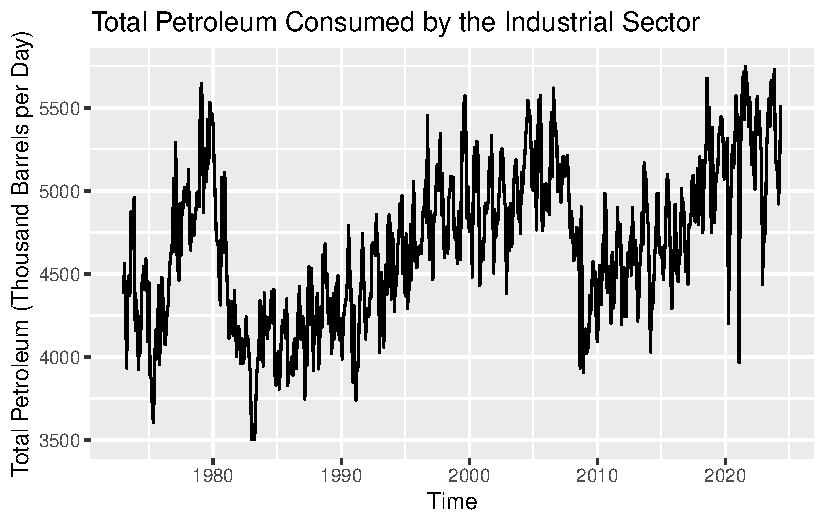
\includegraphics[keepaspectratio]{Report_files/figure-pdf/unnamed-chunk-5-1.pdf}}

According to Figure above, four non-linear upward trends can be observed
during the periods 1975-1980, 1983-2000, 2004-2007, and 2010-2024, as
the intervals of the data movement are not constant, which might be
cyclical. In terms of seasonality, no clear seasonal patterns are
evident, as there are no recurring patterns at fixed intervals.

\subsubsection{Seasonal Plot}\label{seasonal-plot}

\begin{Shaded}
\begin{Highlighting}[]
\DocumentationTok{\#\#\# Seasonal Plot}
\FunctionTok{ggseasonplot}\NormalTok{(industial\_ts) }\SpecialCharTok{+}
  \FunctionTok{ggtitle}\NormalTok{(}\StringTok{"Seasonal Plot of the Total Petroleum Consumed by the Industrial Sector"}\NormalTok{)}\SpecialCharTok{+}
  \FunctionTok{xlab}\NormalTok{(}\StringTok{"Month"}\NormalTok{) }\SpecialCharTok{+} \FunctionTok{ylab}\NormalTok{(}\StringTok{"Total Petroleum (Thousand Barrels per Day)"}\NormalTok{)  }\SpecialCharTok{+}
  \FunctionTok{theme}\NormalTok{(}
    \AttributeTok{legend.text =} \FunctionTok{element\_text}\NormalTok{(}\AttributeTok{size =} \DecValTok{6}\NormalTok{),       }\CommentTok{\# Adjusts the legend text size}
    \AttributeTok{legend.title =} \FunctionTok{element\_text}\NormalTok{(}\AttributeTok{size =} \DecValTok{8}\NormalTok{),      }\CommentTok{\# Adjusts the legend title size}
    \AttributeTok{legend.key.size =} \FunctionTok{unit}\NormalTok{(}\FloatTok{0.5}\NormalTok{, }\StringTok{"lines"}\NormalTok{)       }\CommentTok{\# Shrinks the legend key box size}
\NormalTok{  )}
\end{Highlighting}
\end{Shaded}

\pandocbounded{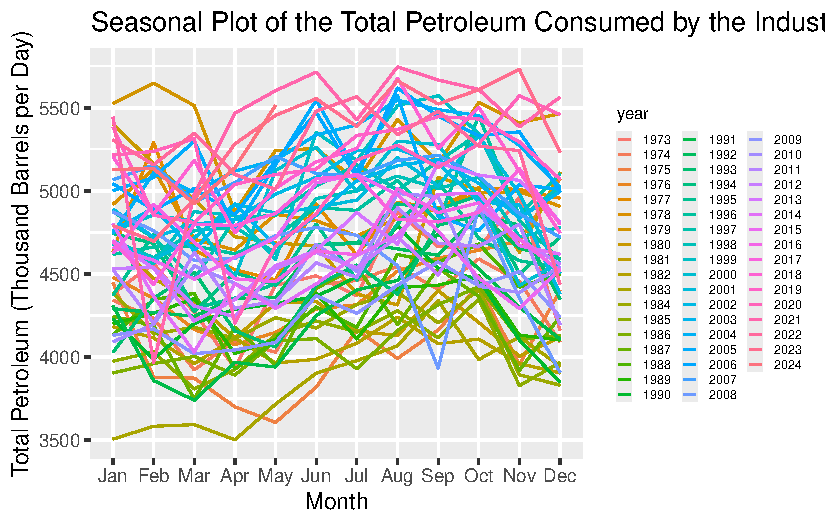
\includegraphics[keepaspectratio]{Report_files/figure-pdf/unnamed-chunk-6-1.pdf}}

As observed in the auto plot, we also do not observe the clear
seasonality in the monthly seasonal plot above. This suggests that the
petroleum consumption in the industrial sector is not influenced by
specific seasons or months. It can also be inferred that the industrial
sector experiences consistent demand throughout the year, regardless of
seasonal factors, likely due to the nature of its projects and
operations.

\subsubsection{ACF Plot}\label{acf-plot}

\begin{Shaded}
\begin{Highlighting}[]
\DocumentationTok{\#\#\# ggAcf}
\FunctionTok{ggAcf}\NormalTok{(industial\_ts) }\SpecialCharTok{+}
  \FunctionTok{ggtitle}\NormalTok{(}\StringTok{"ACF Plot of the Total Petroleum Consumed by the Industrial Sector"}\NormalTok{)}
\end{Highlighting}
\end{Shaded}

\pandocbounded{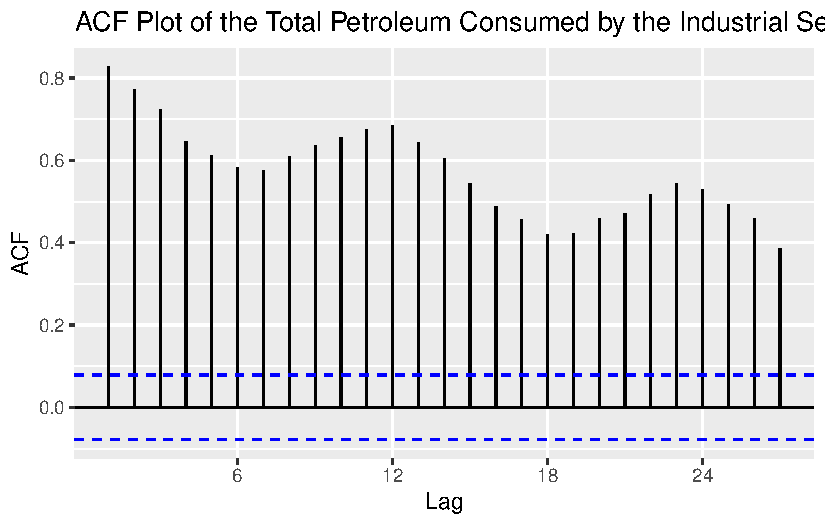
\includegraphics[keepaspectratio]{Report_files/figure-pdf/unnamed-chunk-7-1.pdf}}

The ACF plot of total petroleum consumed by the industrial sector
reveals important characteristics about the time series data. The
significant positive autocorrelation at lag 1 indicates that the current
petroleum consumption is strongly correlated with the consumption from
the previous period. This suggests a high degree of persistence, where
consumption values from one period are closely related to the next. The
gradual decline in autocorrelation over subsequent lags, combined with
the wave-like pattern, points to possible cyclic or seasonal behavior.
The significant spikes that remain above the confidence intervals at
various lags imply that past values up to approximately lag 12 still
influence future consumption patterns, indicating the presence of
long-term dependencies in the data. This suggests that petroleum
consumption in the industrial sector may follow a regular pattern over
time, possibly influenced by recurring industrial activity or demand
cycles.

\subsection{Data Selection}\label{data-selection}

\subsubsection{Modelling Data set}\label{modelling-data-set}

As the current upward trend began in the beginning of 2010, the full
data set is defined from January 2010 to December 2019 until the
pandemic started.

\begin{itemize}
\item
  \textbf{Period}: January 2010 - December 2019
\item
  \textbf{Split Portion}: 80:20 (Training : Test set)
\item
  \textbf{Training set length}: 96months
\item
  \textbf{Test set length}: 24months
\end{itemize}

\begin{Shaded}
\begin{Highlighting}[]
\CommentTok{\# Filter the data to start from 2010 and change the data type to Date}
\NormalTok{industrial\_2010 }\OtherTok{\textless{}{-}}\NormalTok{ industrial }\SpecialCharTok{\%\textgreater{}\%}
  \FunctionTok{filter}\NormalTok{(Month }\SpecialCharTok{\textgreater{}=} \FunctionTok{as.Date}\NormalTok{(}\StringTok{"2010{-}01{-}01"}\NormalTok{))}

\CommentTok{\# Create time series objects from 2010 onwards}
\NormalTok{industrial\_ts\_2010 }\OtherTok{\textless{}{-}} \FunctionTok{ts}\NormalTok{(industrial\_2010[, }\SpecialCharTok{{-}}\DecValTok{1}\NormalTok{], }\AttributeTok{start=}\FunctionTok{c}\NormalTok{(}\DecValTok{2010}\NormalTok{,}\DecValTok{1}\NormalTok{), }\AttributeTok{frequency=}\DecValTok{12}\NormalTok{)}

\CommentTok{\# using precovid data as the Full\_Dataset}
\NormalTok{Full\_Dataset\_industrial }\OtherTok{\textless{}{-}} \FunctionTok{window}\NormalTok{(industrial\_ts\_2010, }\AttributeTok{end=}\FunctionTok{c}\NormalTok{(}\DecValTok{2019}\NormalTok{,}\DecValTok{12}\NormalTok{))}


\DocumentationTok{\#\#\# Industrial Sector}
\NormalTok{train\_industrial }\OtherTok{\textless{}{-}} \FunctionTok{window}\NormalTok{(industrial\_ts\_2010, }\AttributeTok{end =} \FunctionTok{c}\NormalTok{(}\DecValTok{2017}\NormalTok{,}\DecValTok{12}\NormalTok{))}
\NormalTok{test\_industrial }\OtherTok{\textless{}{-}} \FunctionTok{window}\NormalTok{(industrial\_ts\_2010, }\AttributeTok{start =} \FunctionTok{c}\NormalTok{(}\DecValTok{2018}\NormalTok{,}\DecValTok{1}\NormalTok{), }\AttributeTok{end =} \FunctionTok{c}\NormalTok{(}\DecValTok{2019}\NormalTok{,}\DecValTok{12}\NormalTok{))}

\CommentTok{\#check number of observations}
\FunctionTok{length}\NormalTok{(train\_industrial) }\CommentTok{\# 96 (80\%)}
\end{Highlighting}
\end{Shaded}

\begin{verbatim}
[1] 96
\end{verbatim}

\begin{Shaded}
\begin{Highlighting}[]
\FunctionTok{length}\NormalTok{(test\_industrial) }\CommentTok{\# 24 (20\%)}
\end{Highlighting}
\end{Shaded}

\begin{verbatim}
[1] 24
\end{verbatim}

\subsubsection{Covid-19 Data Set}\label{covid-19-data-set}

For this analysis, we focus on the period from January 2010 onward for
all petroleum consumption data in the industrial sector. This timeframe
captures both pre- and post-COVID-19 periods, enabling us to evaluate
the potential shifts caused by the pandemic and external shocks. The
subset of data from January 2010 to April 2024 is named
Full\_Dataset\_Industrial.

The period from 2010 to 2024 was strategically chosen to focus on
contemporary trends, particularly the disruptions caused by the COVID-19
pandemic. While previous global events, such as the Japanese asset price
bubble, the dot-com bubble, and the subprime mortgage crisis, had
profound impacts on economic activity and energy demand, including data
from those periods would likely introduce structural breaks unrelated to
the COVID-19 crisis. Such breaks could complicate the interpretation of
pandemic-specific effects on petroleum consumption. By limiting our
analysis to 2010 onwards, we avoid introducing unrelated outliers or
breaks from earlier periods, ensuring that the results are more focused
on the modern post-COVID energy landscape.

\begin{itemize}
\tightlist
\item
  \textbf{Period}: January 2020 - December 2022
\end{itemize}

\begin{Shaded}
\begin{Highlighting}[]
\NormalTok{Covid\_Period\_industrial }\OtherTok{\textless{}{-}} \FunctionTok{window}\NormalTok{(industrial\_ts\_2010, }\AttributeTok{start =} \FunctionTok{c}\NormalTok{(}\DecValTok{2020}\NormalTok{,}\DecValTok{1}\NormalTok{), }\AttributeTok{end=}\FunctionTok{c}\NormalTok{(}\DecValTok{2024}\NormalTok{,}\DecValTok{5}\NormalTok{))}
\end{Highlighting}
\end{Shaded}

Additionally, the COVID-19 period is defined as January 2021 to December
2022, encompassing both the height of the pandemic and the early
recovery phase. This period is critical for analyzing how the pandemic
altered seasonal trends and consumption behaviors across all three
sectors. By splitting the dataset into pre-COVID (January 2010 to
December 2019) and post-COVID (January 2020 onward) segments, we can
compare these distinct phases. This approach isolates the pandemic's
effects on petroleum consumption while avoiding the noise of unrelated
historical events, thereby enhancing the precision and relevance of our
analysis.

\subsubsection{Plot}\label{plot}

\begin{Shaded}
\begin{Highlighting}[]
\CommentTok{\# Visualization for 2010 onwards}
\FunctionTok{autoplot}\NormalTok{(industrial\_ts\_2010) }\SpecialCharTok{+} 
  \FunctionTok{autolayer}\NormalTok{(train\_industrial, }\AttributeTok{series =} \StringTok{"Training Set"}\NormalTok{) }\SpecialCharTok{+}
  \FunctionTok{autolayer}\NormalTok{(test\_industrial, }\AttributeTok{series =} \StringTok{"Test Set"}\NormalTok{) }\SpecialCharTok{+}
  \FunctionTok{autolayer}\NormalTok{(Covid\_Period\_industrial, }\AttributeTok{series=}\StringTok{"Covid{-}19"}\NormalTok{) }\SpecialCharTok{+}
  \FunctionTok{ggtitle}\NormalTok{(}\StringTok{"Industrial Sector Petroleum Consumption (2010 onwards)"}\NormalTok{) }\SpecialCharTok{+}
  \FunctionTok{ylab}\NormalTok{(}\StringTok{"Petroleum Consumption"}\NormalTok{)}
\end{Highlighting}
\end{Shaded}

\pandocbounded{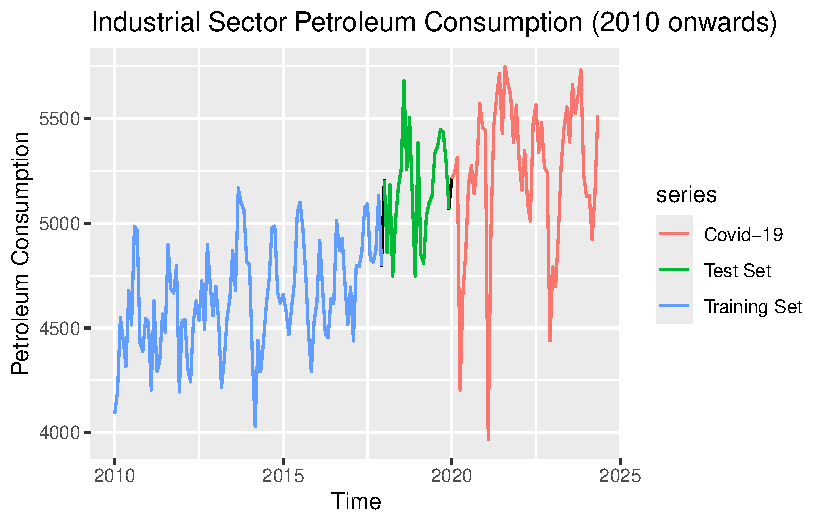
\includegraphics[keepaspectratio]{Report_files/figure-pdf/unnamed-chunk-10-1.pdf}}

\subsection{Data Preparation}\label{data-preparation}

\subsubsection{Stationary Process}\label{stationary-process}

\paragraph{Box-Cox Transformation}\label{box-cox-transformation}

In the above plot, we observe a non-linear upward trend through train
and test dataset, however, we are unable to observe a seasonality since
this data does not show any particular pattern in a fixed duration.
Therefore, we do not consider Box-Cox transformation since the purpose
of the transformation is to simplify the patterns in the historical data
by removing known sources of variation; however, the patterns are
unknown as a clear seasonality does not seems to exist.

\begin{Shaded}
\begin{Highlighting}[]
\DocumentationTok{\#\# Box{-}Cox Transformation}

\CommentTok{\#gain the lambdal value for Industrial industry}
\NormalTok{bc\_lambda2}\OtherTok{\textless{}{-}} \FunctionTok{BoxCox.lambda}\NormalTok{(train\_industrial)}
\NormalTok{bc\_lambda2}
\end{Highlighting}
\end{Shaded}

\begin{verbatim}
[1] 1.999924
\end{verbatim}

\begin{Shaded}
\begin{Highlighting}[]
\CommentTok{\#Do the BC{-} transformation for Industrial industry}
\NormalTok{train\_industrial }\SpecialCharTok{\%\textgreater{}\%}  \FunctionTok{BoxCox}\NormalTok{(}\AttributeTok{lambda=}\NormalTok{ bc\_lambda2) }\SpecialCharTok{\%\textgreater{}\%} \FunctionTok{ggtsdisplay}\NormalTok{()}
\end{Highlighting}
\end{Shaded}

\pandocbounded{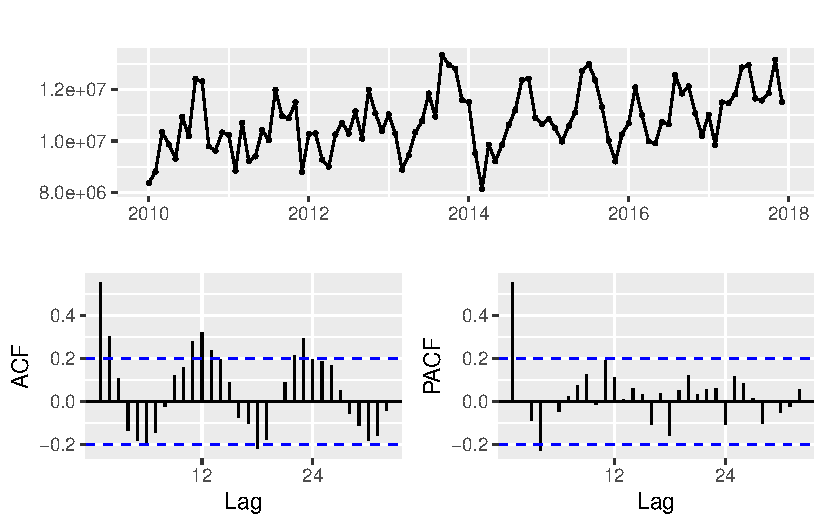
\includegraphics[keepaspectratio]{Report_files/figure-pdf/unnamed-chunk-11-1.pdf}}

\begin{Shaded}
\begin{Highlighting}[]
\CommentTok{\# without BC transformation}
\NormalTok{train\_industrial }\SpecialCharTok{\%\textgreater{}\%} \FunctionTok{ggtsdisplay}\NormalTok{() }
\end{Highlighting}
\end{Shaded}

\pandocbounded{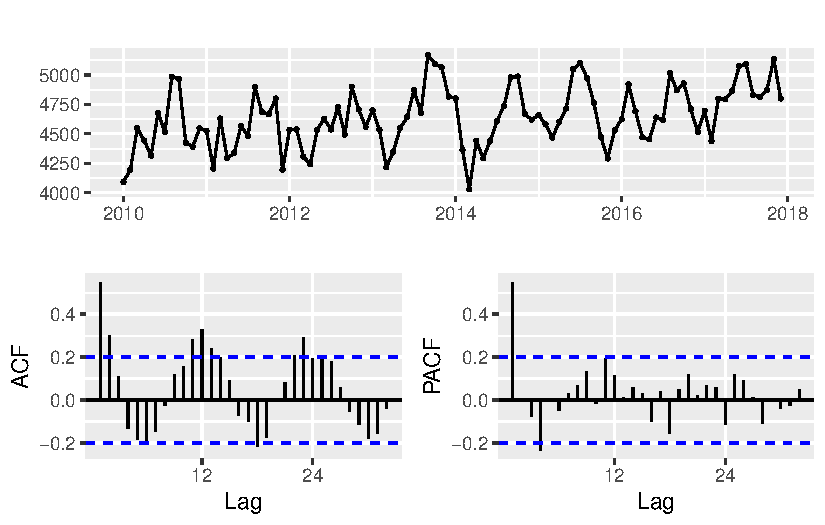
\includegraphics[keepaspectratio]{Report_files/figure-pdf/unnamed-chunk-11-2.pdf}}

Initially, we tried applying the Box-Cox transformation using the lambda
value generated by R, which was 1.999924. However, after comparing the
plots before and after the transformation, we noticed only a slight
change in variance. The difference between the two was negligible. As a
result, we decided not to use the Box-Cox transformation for variance
stabilization. Therefore, we choose to skip the Box-Cox transformation
(Hyndman \& Athanasopoulos, 2021).

\paragraph{Differencing Process}\label{differencing-process}

Next, we focused on stationarity concerning the stability of the mean
and patterns. The primary goal of preparing the dataset for ARIMA
analysis is to transform the data into a stationary process. This means
ensuring that the mean remains constant, the variance is stable, and
there are no predictable patterns over time.

\begin{Shaded}
\begin{Highlighting}[]
\DocumentationTok{\#\# Differencing}

\CommentTok{\#check whether a seasonal difference is needed for industrial industry}
\NormalTok{train\_industrial }\SpecialCharTok{\%\textgreater{}\%} \FunctionTok{nsdiffs}\NormalTok{() }\CommentTok{\# 0: no seasonal differencing is recommended  }
\end{Highlighting}
\end{Shaded}

\begin{verbatim}
[1] 0
\end{verbatim}

\begin{Shaded}
\begin{Highlighting}[]
\NormalTok{train\_industrial }\SpecialCharTok{\%\textgreater{}\%} \FunctionTok{ggtsdisplay}\NormalTok{() }\CommentTok{\# However clear seasonality in ACF and PACF}
\end{Highlighting}
\end{Shaded}

\pandocbounded{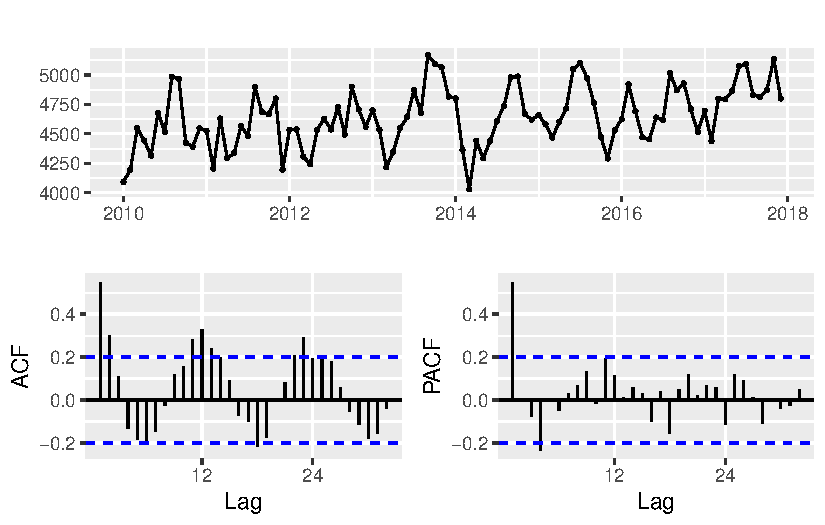
\includegraphics[keepaspectratio]{Report_files/figure-pdf/unnamed-chunk-12-1.pdf}}

In both the PACF and ACF plots, significant autocorrelation at lag 12
was confirmed, indicating the presence of a seasonal pattern in the
data. To verify this, the nsdiffs() function was used to calculate the
seasonal differencing, but the result was displayed as 0. However, due
to the prominent seasonal differencing at lag 12, it was confirmed that
seasonal differencing was necessary. By performing seasonal
differencing, the goal was to eliminate the seasonal structure and
ensure that the mean remained stable over time.

\begin{Shaded}
\begin{Highlighting}[]
\CommentTok{\#check whether a first difference is needed}
\NormalTok{train\_industrial }\SpecialCharTok{\%\textgreater{}\%} \FunctionTok{diff}\NormalTok{(}\AttributeTok{lag=}\DecValTok{12}\NormalTok{) }\SpecialCharTok{\%\textgreater{}\%} \FunctionTok{ndiffs}\NormalTok{() }\CommentTok{\# Additional lag 0 differencing is recommended}
\end{Highlighting}
\end{Shaded}

\begin{verbatim}
[1] 0
\end{verbatim}

\begin{Shaded}
\begin{Highlighting}[]
\CommentTok{\# Result plot}
\NormalTok{train\_industrial }\SpecialCharTok{\%\textgreater{}\%} \FunctionTok{diff}\NormalTok{(}\AttributeTok{lag=}\DecValTok{12}\NormalTok{) }\SpecialCharTok{\%\textgreater{}\%} \FunctionTok{ggtsdisplay}\NormalTok{()}
\end{Highlighting}
\end{Shaded}

\pandocbounded{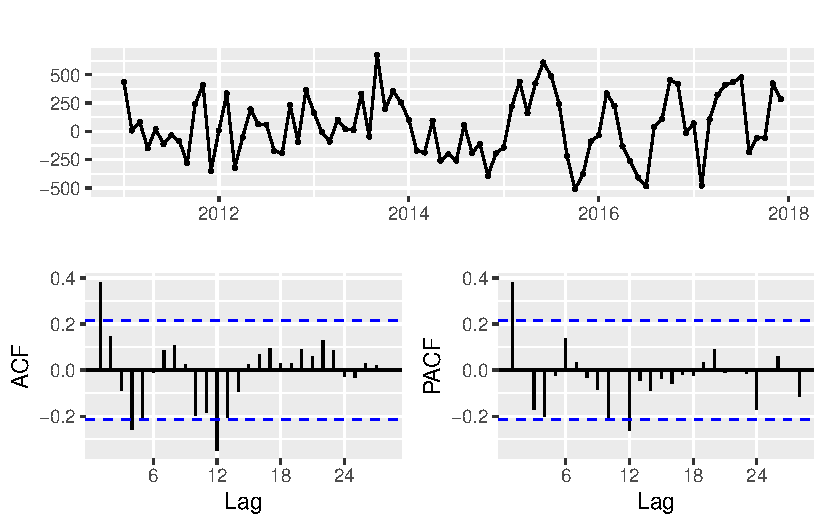
\includegraphics[keepaspectratio]{Report_files/figure-pdf/unnamed-chunk-13-1.pdf}}

Finally, after performing seasonal differencing (lag 12), it was
confirmed that the mean became stable, the variance remained stable, and
no long-term predictable patterns were observed.

At this point, the ndiffs() function was used to check whether
additional differencing was required to stabilize the data. The result
indicated that no further differencing was necessary, confirming that
the data had already reached a stationary state. Therefore, by applying
seasonal differencing at lag 12 (D=1) and no need for first-order
differencing (d=0), the series became stationary with d=0, D=1, and
d+D=1.

\subsection{Model Selection}\label{model-selection}

\subsubsection{Pure AR Model}\label{pure-ar-model}

\begin{Shaded}
\begin{Highlighting}[]
\CommentTok{\# pure AR model(1): ARIMA(1,0,0)(1,1,0)[12]}
\NormalTok{fit\_industrial1 }\OtherTok{\textless{}{-}} \FunctionTok{Arima}\NormalTok{(train\_industrial, }\AttributeTok{order =} \FunctionTok{c}\NormalTok{(}\DecValTok{1}\NormalTok{,}\DecValTok{0}\NormalTok{,}\DecValTok{0}\NormalTok{), }\AttributeTok{season =} \FunctionTok{c}\NormalTok{(}\DecValTok{1}\NormalTok{,}\DecValTok{1}\NormalTok{,}\DecValTok{0}\NormalTok{))}
\end{Highlighting}
\end{Shaded}

For the AR model in the industrial sector, upon analysing the PACF plot,
significant spikes were observed at lag 1, which suggest a non-seasonal
AR (1) model component (p=1). Also, there is a spike in the PACF at lag
12, but not at lag 24. This suggests a seasonal AR (0) model component
(P=1). All these led us to construct an ARIMA (1,0,0) (1,1,0) {[}12{]}
model, which involves a seasonal differencing (d=0, D=1) .

\paragraph{Ljung-Box Test}\label{ljung-box-test}

\begin{Shaded}
\begin{Highlighting}[]
\CommentTok{\# ljung{-}box test}
\FunctionTok{checkresiduals}\NormalTok{(fit\_industrial1) }\CommentTok{\# ARIMA(1,0,0)(1,1,0)[12]: Pass}
\end{Highlighting}
\end{Shaded}

\pandocbounded{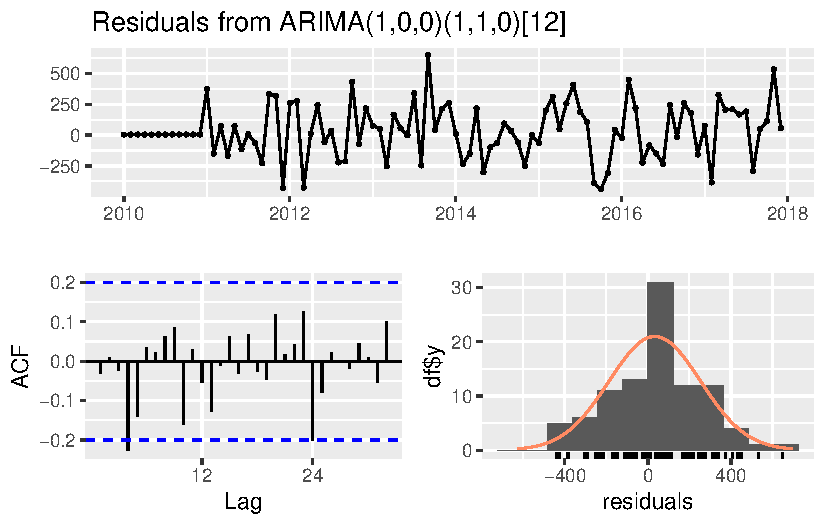
\includegraphics[keepaspectratio]{Report_files/figure-pdf/unnamed-chunk-15-1.pdf}}

\begin{verbatim}

    Ljung-Box test

data:  Residuals from ARIMA(1,0,0)(1,1,0)[12]
Q* = 15.338, df = 17, p-value = 0.5711

Model df: 2.   Total lags used: 19
\end{verbatim}

We will use the checkresiduals() function to verify if the residuals of
these models meet the criteria for white noise by ljung-box test.

\begin{itemize}
\item
  H0: There is no autocorrelation in the residuals.
\item
  H1: At least one of the autocorrelations in the residuals up to 19
  lags.
\end{itemize}

For the pure AR model, the mean of the residual appears to be close to
zero, and the variance seems to be constant. Additionally, according to
the results of the Ljung-Box test, the p-value for fit\_industry1 is
0.5711. Since the p-value is more than 0.05, there is insufficient
evidence to reject the null hypothesis that there is no autocorrelation
in the residuals, indicating that the residuals can be considered white
noise. Therefore, re-identification is not necessary for the model.

\subsubsection{Pure MA Model}\label{pure-ma-model}

For the pure MA model, we examine the ACF plot and find spikes at lag 1
and 4, indicating a non-seasonal MA (1) model with component (q=1). This
pure MA model also does not have a seasonal model since the ACF plot
does not show any spikes at 12 and 24. Consequently, we can build an
ARIMA (0,0,1)(0,1,1){[}12{]} model.

\paragraph{Ljung-Box Test}\label{ljung-box-test-1}

\begin{Shaded}
\begin{Highlighting}[]
\CommentTok{\# ljung{-}box test}
\FunctionTok{checkresiduals}\NormalTok{(fit\_industrial2) }\CommentTok{\# ARIMA(0,0,1)(0,1,1)[12]: Pass}
\end{Highlighting}
\end{Shaded}

\pandocbounded{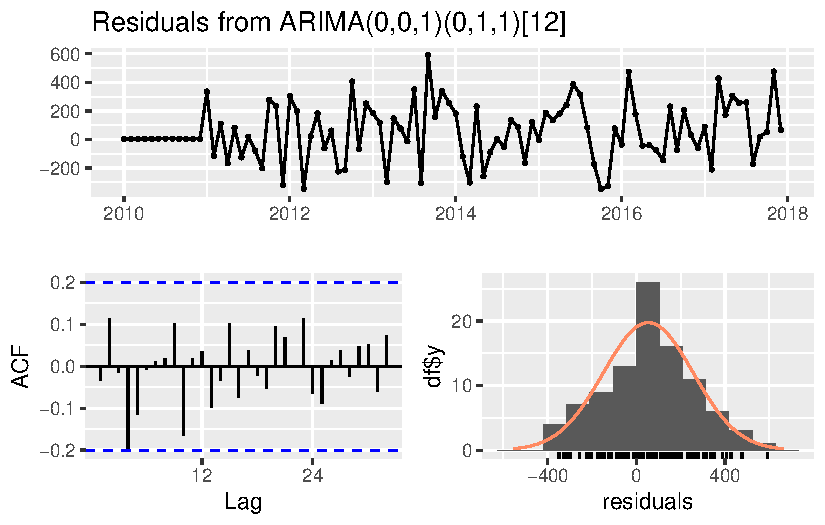
\includegraphics[keepaspectratio]{Report_files/figure-pdf/unnamed-chunk-17-1.pdf}}

\begin{verbatim}

    Ljung-Box test

data:  Residuals from ARIMA(0,0,1)(0,1,1)[12]
Q* = 14.78, df = 17, p-value = 0.6113

Model df: 2.   Total lags used: 19
\end{verbatim}

We will use the checkresiduals() function to verify if the residuals of
these models meet the criteria for white noise by ljung-box test.

\begin{itemize}
\item
  H0: There is no autocorrelation in the residuals.
\item
  H1: At least one of the autocorrelations in the residuals up to 19
  lags.
\end{itemize}

For pure MA model, the mean of the residual appears to be close to zero,
and the variance seems to be constant. Additionally, according to the
results of the Ljung-Box test, the p-value for fit\_industry2 is
0.6113.~ The p-value is more than 0.05, there is insufficient evidence
to reject the null hypothesis, indicating that the residuals can be
considered white noise, which does not require to reidentify the model.

\subsubsection{Auto ARIMA Model}\label{auto-arima-model}

For auto ARIMA model, we used the auto.arima() function to build another
ARIMA model. The result suggests ARIMA(1,1,1)(1,0,0){[}12{]}, denoted as
`auto\_arima\_industrial'.

\paragraph{Ljung-Test}\label{ljung-test}

\begin{Shaded}
\begin{Highlighting}[]
\CommentTok{\# ljung box test}
\FunctionTok{checkresiduals}\NormalTok{(auto\_arima\_industrial)}
\end{Highlighting}
\end{Shaded}

\pandocbounded{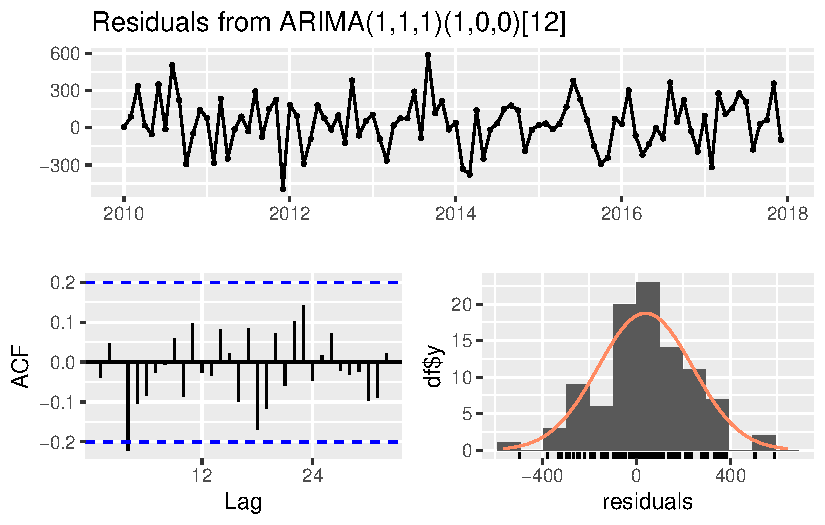
\includegraphics[keepaspectratio]{Report_files/figure-pdf/unnamed-chunk-19-1.pdf}}

\begin{verbatim}

    Ljung-Box test

data:  Residuals from ARIMA(1,1,1)(1,0,0)[12]
Q* = 17.596, df = 16, p-value = 0.3481

Model df: 3.   Total lags used: 19
\end{verbatim}

The residuals of the ARIMA(1,1,1)(1,0,0){[}12{]} model exhibit a zero
mean and constant variance, aligning with some of the assumptions of a
well-behaved residual series. The histogram of the residuals shows that
they are approximately normally distributed, indicating that the
residuals are symmetrically centered around zero without significant
skewness or kurtosis. To statistically evaluate the presence of
autocorrelation in the residuals, we conducted the following hypothesis
test:

H₀: There is no autocorrelation in the residuals.

H₁: At least one of the autocorrelations in the residuals is
significant.

Using the Ljung-Box test, the p-value obtained was 0.3481, which is
considerably higher than the conventional significance level of α = 0.05
(Appendix 19. Therefore, we do not reject the null hypothesis. As a
result, there is insufficient evidence to conclude that the residuals
are not white noise.

\subsubsection{Auto ETS Model}\label{auto-ets-model}

\begin{Shaded}
\begin{Highlighting}[]
\DocumentationTok{\#\# Auto ets model}
\CommentTok{\# develop auto ets model}
\NormalTok{auto\_ets\_industrial }\OtherTok{\textless{}{-}} \FunctionTok{ets}\NormalTok{(train\_industrial) }\CommentTok{\# ETS(M,A,A)}

\CommentTok{\# Check the result}
\FunctionTok{summary}\NormalTok{(auto\_ets\_industrial)}
\end{Highlighting}
\end{Shaded}

\begin{verbatim}
ETS(M,A,A) 

Call:
ets(y = train_industrial)

  Smoothing parameters:
    alpha = 5e-04 
    beta  = 1e-04 
    gamma = 1e-04 

  Initial states:
    l = 4482.3407 
    b = 3.3537 
    s = -100.848 55.7088 152.6431 220.2689 235.5492 59.1909
           56.5035 -121.7612 -193.2253 -173.1783 -137.3123 -53.5393

  sigma:  0.0438

     AIC     AICc      BIC 
1475.251 1483.097 1518.845 

Training set error measures:
                   ME    RMSE      MAE        MPE     MAPE      MASE      ACF1
Training set -2.46755 186.543 154.9604 -0.2125913 3.346057 0.6882641 0.3167086
\end{verbatim}

Next, we used the ets() function in R to automatically select an
appropriate ETS model. The result was the ETS(M,A,A) model. Here, ``M''
indicates multiplicative errors, meaning that forecast errors are
proportional to the level of the time series. ``A'' denotes an additive
trend, indicating that a long-term trend is considered in the data. The
final ``A'' indicates additive seasonality. This model is well-suited
for capturing the multiplicative nature of errors and the additive trend
and seasonality in the data.

\paragraph{Ljung-Box Test}\label{ljung-box-test-2}

\begin{Shaded}
\begin{Highlighting}[]
\CommentTok{\# ljunb{-}box test}
\FunctionTok{checkresiduals}\NormalTok{(auto\_ets\_industrial)}
\end{Highlighting}
\end{Shaded}

\pandocbounded{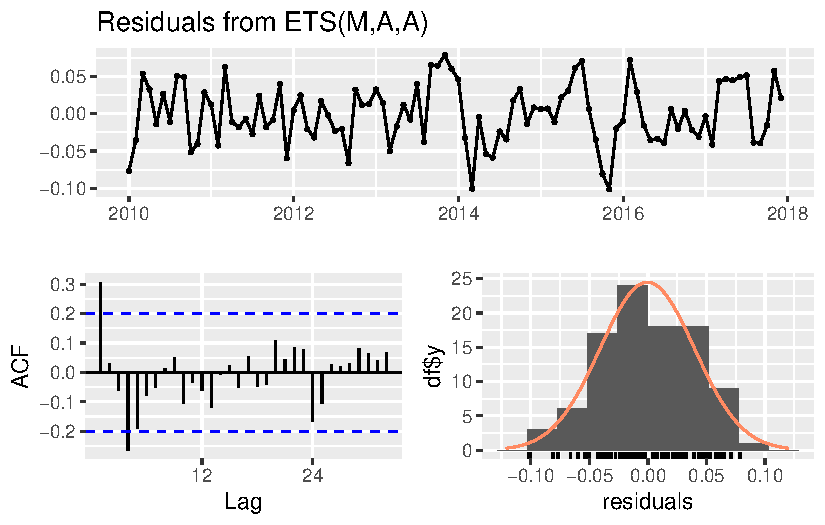
\includegraphics[keepaspectratio]{Report_files/figure-pdf/unnamed-chunk-21-1.pdf}}

\begin{verbatim}

    Ljung-Box test

data:  Residuals from ETS(M,A,A)
Q* = 26.639, df = 19, p-value = 0.1134

Model df: 0.   Total lags used: 19
\end{verbatim}

The residuals of the ETS(M,A,A) model exhibit a zero mean and constant
variance, aligning with some of the assumptions of a well-behaved
residual series. The histogram of the residuals indicates that they are
approximately normally distributed, suggesting that the residuals are
symmetrically centered around zero, with no significant skewness or
kurtosis. However, spikes are observed at the first and fourth lags in
the ACF plot. Next, we performed the following hypothesis test to
statistically evaluate the presence of autocorrelation in the residuals:

H₀: There is no autocorrelation in the residuals.

H₁: At least one of the autocorrelations in the residuals is significant
up to lag 19

Using the Ljung-Box test, the p-value associated with this test was
0.1134, which is higher than the conventional significance level of α =
0.05. As a result, we could not reject the null hypothesis, meaning that
there is no evidence of significant autocorrelation in the residuals up
to lag 19.

\subsection{Model Evaluation}\label{model-evaluation}

\subsubsection{Forecast Interval}\label{forecast-interval}

\paragraph{Pure AR vs Pure MA Model}\label{pure-ar-vs-pure-ma-model}

For 𝑑=0 and 𝐷=1 ARIMA models we have, because there is no clear trend
for a long-term in the data after differencing based on time series plot
in Figure, therefore it is not necessary to retain the constant term.
Therefore, at this stage, we estimated two pure ARIMA models using the
training dataset for the Industrial sector without including constants.
Two forecast model we have now are:

\begin{itemize}
\item
  ARIMA (1,0,0)(1,1,0){[}12{]} without constant, denoted as '
  fit\_industry1'
\item
  ARIMA (0,0,1)(0,1,1){[}12{]} without constant, denoted as '
  fit\_industry2'
\end{itemize}

\begin{Shaded}
\begin{Highlighting}[]
\CommentTok{\# forecast}
\NormalTok{fc1\_industrial }\OtherTok{\textless{}{-}} \FunctionTok{forecast}\NormalTok{(fit\_industrial1, }\AttributeTok{h=}\FunctionTok{length}\NormalTok{(test\_industrial)) }\CommentTok{\# AR}
\NormalTok{fc2\_industrial }\OtherTok{\textless{}{-}} \FunctionTok{forecast}\NormalTok{(fit\_industrial2, }\AttributeTok{h=}\FunctionTok{length}\NormalTok{(test\_industrial)) }\CommentTok{\# MA}

\CommentTok{\# Autoplot}
\FunctionTok{autoplot}\NormalTok{(Full\_Dataset\_industrial) }\SpecialCharTok{+} 
  \FunctionTok{autolayer}\NormalTok{(fc1\_industrial, }\AttributeTok{series =}  \StringTok{"Pure AR Model"}\NormalTok{, }
            \AttributeTok{alpha =} \FloatTok{0.5}\NormalTok{) }\SpecialCharTok{+}
  \FunctionTok{autolayer}\NormalTok{(fc2\_industrial, }\AttributeTok{series =}  \StringTok{"Pure MA Model"}\NormalTok{, }
            \AttributeTok{alpha =} \FloatTok{0.5}\NormalTok{) }\SpecialCharTok{+}
  \FunctionTok{ggtitle}\NormalTok{(}\StringTok{"Forecasts of pure AR/MA models for Industrial Sector"}\NormalTok{) }\SpecialCharTok{+}
  \FunctionTok{xlab}\NormalTok{(}\StringTok{"Time"}\NormalTok{) }\SpecialCharTok{+} \FunctionTok{ylab}\NormalTok{(}\StringTok{"Total Petroleum (Thousand Barrels per Day)"}\NormalTok{)}
\end{Highlighting}
\end{Shaded}

\pandocbounded{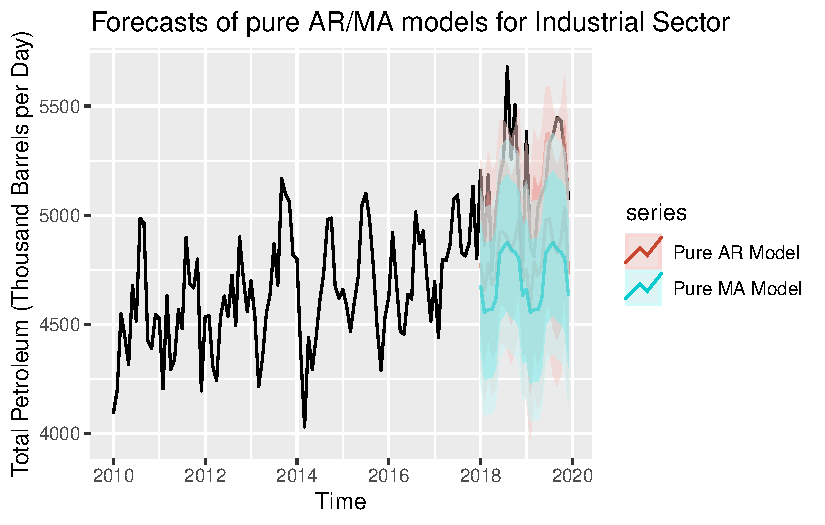
\includegraphics[keepaspectratio]{Report_files/figure-pdf/unnamed-chunk-22-1.pdf}}

After the residuals check, we conduct 2 forecasts for test data of the
industrial sector by using fc1\_Industrial, fc2\_Industrial. According
to the forecast plot with the actual test data below in figure below,
the forecast intervals are all within a reasonable range. Therefore, we
proceed to examine the model's goodness of fit \& forecast accuracy.

\subparagraph{Summary}\label{summary}

\begin{Shaded}
\begin{Highlighting}[]
\CommentTok{\# summary }
\FunctionTok{summary}\NormalTok{(fc1\_industrial)}
\end{Highlighting}
\end{Shaded}

\begin{verbatim}

Forecast method: ARIMA(1,0,0)(1,1,0)[12]

Model Information:
Series: train_industrial 
ARIMA(1,0,0)(1,1,0)[12] 

Coefficients:
         ar1     sar1
      0.3891  -0.3569
s.e.  0.1024   0.1121

sigma^2 = 57674:  log likelihood = -579.5
AIC=1165.01   AICc=1165.31   BIC=1172.3

Error measures:
                   ME    RMSE      MAE       MPE     MAPE      MASE        ACF1
Training set 33.22599 221.954 169.8269 0.5895324 3.643139 0.7542945 -0.03080685

Forecasts:
         Point Forecast    Lo 80    Hi 80    Lo 95    Hi 95
Jan 2018       4779.258 4471.487 5087.029 4308.563 5249.953
Feb 2018       4652.445 4322.193 4982.697 4147.368 5157.522
Mar 2018       4776.570 4443.046 5110.094 4266.489 5286.651
Apr 2018       4684.107 4350.090 5018.124 4173.272 5194.941
May 2018       4719.767 4385.676 5053.859 4208.819 5230.716
Jun 2018       4919.661 4585.559 5253.764 4408.696 5430.627
Jul 2018       4922.806 4588.702 5256.910 4411.838 5433.775
Aug 2018       4895.864 4561.760 5229.969 4384.896 5406.833
Sep 2018       4833.283 4499.178 5167.387 4322.314 5344.251
Oct 2018       4891.257 4557.152 5225.361 4380.288 5402.226
Nov 2018       4981.479 4647.374 5315.584 4470.510 5492.448
Dec 2018       4698.408 4364.304 5032.513 4187.440 5209.377
Jan 2019       4749.500 4361.169 5137.831 4155.598 5343.402
Feb 2019       4576.087 4180.191 4971.983 3970.617 5181.557
Mar 2019       4784.091 4387.063 5181.120 4176.888 5391.294
Apr 2019       4722.857 4325.657 5120.057 4115.392 5330.321
May 2019       4771.117 4373.891 5168.342 4163.612 5378.621
Jun 2019       4974.846 4577.616 5372.075 4367.336 5582.356
Jul 2019       4983.437 4586.207 5380.667 4375.926 5590.948
Aug 2019       4872.239 4475.009 5269.470 4264.728 5479.751
Sep 2019       4826.179 4428.949 5223.409 4218.668 5433.690
Oct 2019       4884.017 4486.787 5281.248 4276.506 5491.529
Nov 2019       5035.522 4638.291 5432.752 4428.010 5643.033
Dec 2019       4734.690 4337.460 5131.920 4127.179 5342.201
\end{verbatim}

\begin{Shaded}
\begin{Highlighting}[]
\FunctionTok{summary}\NormalTok{(fc2\_industrial)}
\end{Highlighting}
\end{Shaded}

\begin{verbatim}

Forecast method: ARIMA(0,0,1)(0,1,1)[12]

Model Information:
Series: train_industrial 
ARIMA(0,0,1)(0,1,1)[12] 

Coefficients:
         ma1     sma1
      0.3888  -0.6678
s.e.  0.0986   0.1618

sigma^2 = 51053:  log likelihood = -577.1
AIC=1160.2   AICc=1160.5   BIC=1167.49

Error measures:
                   ME     RMSE     MAE      MPE     MAPE      MASE        ACF1
Training set 53.97469 208.8253 162.714 1.030037 3.475568 0.7227021 -0.03326999

Forecasts:
         Point Forecast    Lo 80    Hi 80    Lo 95    Hi 95
Jan 2018       4677.180 4387.468 4966.892 4234.104 5120.256
Feb 2018       4554.866 4244.046 4865.686 4079.507 5030.224
Mar 2018       4566.739 4255.919 4877.559 4091.380 5042.097
Apr 2018       4566.831 4256.011 4877.651 4091.472 5042.189
May 2018       4615.104 4304.284 4925.924 4139.745 5090.462
Jun 2018       4823.460 4512.640 5134.280 4348.102 5298.819
Jul 2018       4852.433 4541.613 5163.253 4377.074 5327.791
Aug 2018       4875.338 4564.517 5186.158 4399.979 5350.696
Sep 2018       4843.729 4532.909 5154.549 4368.371 5319.087
Oct 2018       4830.795 4519.975 5141.615 4355.437 5306.154
Nov 2018       4801.344 4490.523 5112.164 4325.985 5276.702
Dec 2018       4631.361 4320.551 4942.172 4156.018 5106.705
Jan 2019       4659.661 4334.301 4985.020 4162.066 5157.255
Feb 2019       4554.866 4227.356 4882.376 4053.982 5055.749
Mar 2019       4566.739 4239.229 4894.249 4065.855 5067.622
Apr 2019       4566.831 4239.321 4894.341 4065.947 5067.714
May 2019       4615.104 4287.594 4942.614 4114.220 5115.987
Jun 2019       4823.460 4495.950 5150.970 4322.577 5324.344
Jul 2019       4852.433 4524.923 5179.943 4351.549 5353.316
Aug 2019       4875.338 4547.827 5202.848 4374.454 5376.221
Sep 2019       4843.729 4516.219 5171.239 4342.845 5344.612
Oct 2019       4830.795 4503.285 5158.305 4329.912 5331.679
Nov 2019       4801.344 4473.834 5128.854 4300.460 5302.227
Dec 2019       4631.361 4303.860 4958.862 4130.492 5132.230
\end{verbatim}

\paragraph{Auto ETS vs Auto ARIMA
Model}\label{auto-ets-vs-auto-arima-model}

\begin{Shaded}
\begin{Highlighting}[]
\CommentTok{\# forecast}
\NormalTok{fc\_ets\_industrial }\OtherTok{\textless{}{-}} \FunctionTok{forecast}\NormalTok{(auto\_ets\_industrial, }\AttributeTok{h =} \FunctionTok{length}\NormalTok{(test\_industrial))}
\NormalTok{fc\_arima\_industrial }\OtherTok{\textless{}{-}} \FunctionTok{forecast}\NormalTok{(auto\_arima\_industrial, }\AttributeTok{h=}\FunctionTok{length}\NormalTok{(test\_industrial))}

\CommentTok{\# Autoplot}
\FunctionTok{autoplot}\NormalTok{(Full\_Dataset\_industrial) }\SpecialCharTok{+} 
  \FunctionTok{autolayer}\NormalTok{(fc\_ets\_industrial, }\AttributeTok{series =}  \StringTok{"Auto ETS Model"}\NormalTok{, }
            \AttributeTok{alpha =} \FloatTok{0.5}\NormalTok{) }\SpecialCharTok{+}
  \FunctionTok{autolayer}\NormalTok{(fc\_arima\_industrial, }\AttributeTok{series =}  \StringTok{"Auto ARIMA Model"}\NormalTok{, }
            \AttributeTok{alpha =} \FloatTok{0.5}\NormalTok{) }\SpecialCharTok{+}
  \FunctionTok{ggtitle}\NormalTok{(}\StringTok{"Forecasts of auto ETS and ARIMA models for Industrial Sector"}\NormalTok{) }\SpecialCharTok{+}
  \FunctionTok{xlab}\NormalTok{(}\StringTok{"Time"}\NormalTok{) }\SpecialCharTok{+} \FunctionTok{ylab}\NormalTok{(}\StringTok{"Total Petroleum (Thousand Barrels per Day)"}\NormalTok{)}
\end{Highlighting}
\end{Shaded}

\pandocbounded{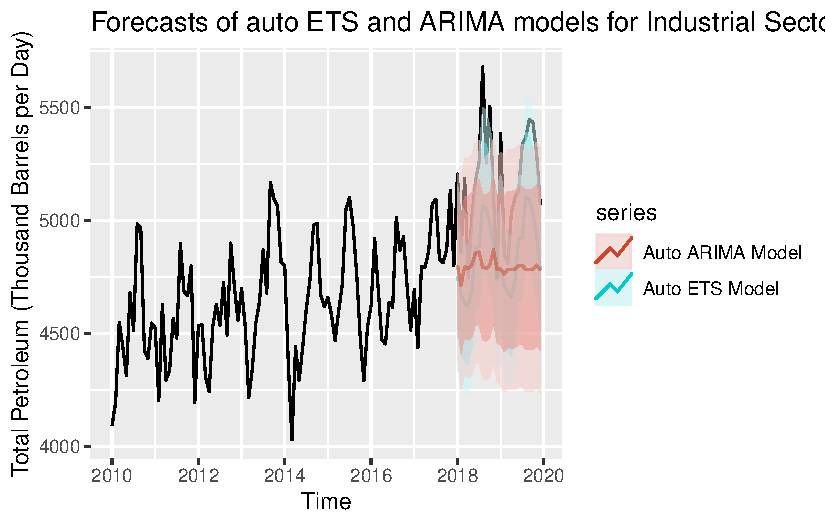
\includegraphics[keepaspectratio]{Report_files/figure-pdf/unnamed-chunk-24-1.pdf}}

We conduct 2 forecasts for test data of the industrial sector by using
the auto ETS and auto ARIMA models. According to the forecast plot with
the actual test data below in figure, the forecast intervals are all
within a reasonable range. Therefore, we proceed to examine the model's
goodness of fit \& forecast accuracy.

\subparagraph{Summary}\label{summary-1}

\begin{Shaded}
\begin{Highlighting}[]
\FunctionTok{summary}\NormalTok{(fc\_ets\_industrial)}
\end{Highlighting}
\end{Shaded}

\begin{verbatim}

Forecast method: ETS(M,A,A)

Model Information:
ETS(M,A,A) 

Call:
ets(y = train_industrial)

  Smoothing parameters:
    alpha = 5e-04 
    beta  = 1e-04 
    gamma = 1e-04 

  Initial states:
    l = 4482.3407 
    b = 3.3537 
    s = -100.848 55.7088 152.6431 220.2689 235.5492 59.1909
           56.5035 -121.7612 -193.2253 -173.1783 -137.3123 -53.5393

  sigma:  0.0438

     AIC     AICc      BIC 
1475.251 1483.097 1518.845 

Error measures:
                   ME    RMSE      MAE        MPE     MAPE      MASE      ACF1
Training set -2.46755 186.543 154.9604 -0.2125913 3.346057 0.6882641 0.3167086

Forecasts:
         Point Forecast    Lo 80    Hi 80    Lo 95    Hi 95
Jan 2018       4751.647 4484.664 5018.631 4343.332 5159.963
Feb 2018       4671.183 4408.721 4933.645 4269.781 5072.584
Mar 2018       4638.664 4378.029 4899.300 4240.058 5037.271
Apr 2018       4621.955 4362.259 4881.652 4224.784 5019.126
May 2018       4696.731 4432.834 4960.629 4293.135 5100.328
Jun 2018       4878.348 4604.245 5152.450 4459.144 5297.551
Jul 2018       4884.371 4609.930 5158.812 4464.649 5304.092
Aug 2018       5064.015 4779.480 5348.550 4628.857 5499.174
Sep 2018       5052.064 4768.200 5335.928 4617.932 5486.196
Oct 2018       4987.781 4707.529 5268.034 4559.173 5416.390
Nov 2018       4894.194 4619.200 5169.188 4473.627 5314.761
Dec 2018       4740.972 4474.587 5007.357 4333.571 5148.373
Jan 2019       4791.607 4522.376 5060.837 4379.854 5203.359
Feb 2019       4711.142 4446.432 4975.852 4306.303 5115.981
Mar 2019       4678.624 4415.741 4941.507 4276.579 5080.669
Apr 2019       4661.915 4399.970 4923.860 4261.304 5062.525
May 2019       4736.691 4470.544 5002.838 4329.654 5143.728
Jun 2019       4918.307 4641.955 5194.659 4495.663 5340.951
Jul 2019       4924.330 4647.639 5201.021 4501.168 5347.493
Aug 2019       5103.975 4817.189 5390.760 4665.374 5542.575
Sep 2019       5092.023 4805.909 5378.138 4654.449 5529.598
Oct 2019       5027.741 4745.237 5310.245 4595.689 5459.793
Nov 2019       4934.154 4656.907 5211.400 4510.142 5358.165
Dec 2019       4780.931 4512.292 5049.570 4370.084 5191.778
\end{verbatim}

\begin{Shaded}
\begin{Highlighting}[]
\FunctionTok{summary}\NormalTok{(fc\_arima\_industrial)}
\end{Highlighting}
\end{Shaded}

\begin{verbatim}

Forecast method: ARIMA(1,1,1)(1,0,0)[12]

Model Information:
Series: train_industrial 
ARIMA(1,1,1)(1,0,0)[12] 

Coefficients:
         ar1      ma1    sar1
      0.4899  -0.9576  0.2546
s.e.  0.1000   0.0301  0.1097

sigma^2 = 43345:  log likelihood = -641.42
AIC=1290.83   AICc=1291.28   BIC=1301.05

Error measures:
                   ME     RMSE      MAE       MPE     MAPE      MASE
Training set 38.84992 203.8108 159.2547 0.6726174 3.417933 0.7073376
                    ACF1
Training set -0.03794146

Forecasts:
         Point Forecast    Lo 80    Hi 80    Lo 95    Hi 95
Jan 2018       4801.389 4534.576 5068.202 4393.334 5209.444
Feb 2018       4713.968 4411.703 5016.232 4251.694 5176.241
Mar 2018       4794.694 4481.789 5107.599 4316.147 5273.241
Apr 2018       4788.176 4471.150 5105.203 4303.326 5273.027
May 2018       4803.672 4484.576 5122.768 4315.656 5291.687
Jun 2018       4856.046 4535.627 5176.466 4366.007 5346.086
Jul 2018       4860.115 4538.677 5181.553 4368.518 5351.713
Aug 2018       4792.841 4470.520 5115.163 4299.893 5285.789
Sep 2018       4788.545 4465.404 5111.686 4294.343 5282.746
Oct 2018       4803.137 4479.208 5127.066 4307.730 5298.544
Nov 2018       4869.796 4545.094 5194.497 4373.208 5366.384
Dec 2018       4785.028 4459.563 5110.493 4287.272 5282.784
Jan 2019       4785.357 4447.631 5123.084 4268.849 5301.865
Feb 2019       4763.093 4420.358 5105.828 4238.925 5287.261
Mar 2019       4783.646 4438.249 5129.043 4255.407 5311.885
Apr 2019       4781.986 4434.803 5129.168 4251.016 5312.956
May 2019       4785.931 4437.329 5134.533 4252.790 5319.072
Jun 2019       4799.267 4449.411 5149.123 4264.208 5334.326
Jul 2019       4800.303 4449.271 5151.334 4263.447 5337.159
Aug 2019       4783.173 4431.006 5135.340 4244.580 5321.765
Sep 2019       4782.079 4428.797 5135.360 4241.781 5322.376
Oct 2019       4785.794 4431.410 5140.179 4243.810 5327.779
Nov 2019       4802.768 4447.288 5158.248 4259.108 5346.427
Dec 2019       4781.183 4424.613 5137.753 4235.856 5326.510
\end{verbatim}

\subsubsection{Goodness of Fit}\label{goodness-of-fit}

\begin{Shaded}
\begin{Highlighting}[]
\CommentTok{\# Goodness of Fit}
\NormalTok{GoF }\OtherTok{\textless{}{-}} \FunctionTok{data.frame}\NormalTok{(}\AttributeTok{AIC =} \FunctionTok{c}\NormalTok{(fit\_industrial1}\SpecialCharTok{$}\NormalTok{aic, }
\NormalTok{                          fit\_industrial2}\SpecialCharTok{$}\NormalTok{aic, }
\NormalTok{                          auto\_ets\_industrial}\SpecialCharTok{$}\NormalTok{aic, }
\NormalTok{                          auto\_arima\_industrial}\SpecialCharTok{$}\NormalTok{aic),}
                  \AttributeTok{AICc =} \FunctionTok{c}\NormalTok{(fit\_industrial1}\SpecialCharTok{$}\NormalTok{aicc, }
\NormalTok{                           fit\_industrial2}\SpecialCharTok{$}\NormalTok{aicc, }
\NormalTok{                           auto\_ets\_industrial}\SpecialCharTok{$}\NormalTok{aicc, }
\NormalTok{                           auto\_arima\_industrial}\SpecialCharTok{$}\NormalTok{aicc),}
                  \AttributeTok{BIC =} \FunctionTok{c}\NormalTok{(fit\_industrial1}\SpecialCharTok{$}\NormalTok{bic, }
\NormalTok{                          fit\_industrial2}\SpecialCharTok{$}\NormalTok{bic, }
\NormalTok{                          auto\_ets\_industrial}\SpecialCharTok{$}\NormalTok{bic, }
\NormalTok{                          auto\_arima\_industrial}\SpecialCharTok{$}\NormalTok{bic))}

\CommentTok{\# Define row names}
\FunctionTok{row.names}\NormalTok{(GoF) }\OtherTok{\textless{}{-}} \FunctionTok{c}\NormalTok{(}\StringTok{"Pure AR"}\NormalTok{, }\StringTok{"Pure MA"}\NormalTok{, }\StringTok{"Auto ETS"}\NormalTok{, }\StringTok{"Auto ARIMA"}\NormalTok{)}

\FunctionTok{print}\NormalTok{(GoF)}
\end{Highlighting}
\end{Shaded}

\begin{verbatim}
                AIC     AICc      BIC
Pure AR    1165.008 1165.308 1172.301
Pure MA    1160.196 1160.496 1167.488
Auto ETS   1475.251 1483.097 1518.845
Auto ARIMA 1290.832 1291.276 1301.047
\end{verbatim}

According to the table, when comparing AICc, AIC, and BIC, the Pure MA
Model that is ARIMA (0,0,1)(0,1,1){[}12{]} model has the lowest scores
compared to the other models in all metrics. Therefore, from the
perspective of goodness of fit, the ARIMA (0,0,1)(0,1,1){[}12{]} model
is more good of fit.

\subsubsection{Accuracy of Models (Traditional
Approach)}\label{accuracy-of-models-traditional-approach}

\subparagraph{Pure AR Model}\label{pure-ar-model-1}

\begin{Shaded}
\begin{Highlighting}[]
\FunctionTok{accuracy}\NormalTok{(fc1\_industrial, test\_industrial)}
\end{Highlighting}
\end{Shaded}

\begin{verbatim}
                    ME     RMSE      MAE       MPE     MAPE      MASE
Training set  33.22599 221.9540 169.8269 0.5895324 3.643139 0.7542945
Test set     347.82950 397.9014 347.8295 6.5917793 6.591779 1.5449017
                    ACF1 Theil's U
Training set -0.03080685        NA
Test set      0.05477409  1.304118
\end{verbatim}

\subparagraph{Pure MA Model}\label{pure-ma-model-1}

\begin{Shaded}
\begin{Highlighting}[]
\FunctionTok{accuracy}\NormalTok{(fc2\_industrial, test\_industrial)}
\end{Highlighting}
\end{Shaded}

\begin{verbatim}
                    ME     RMSE      MAE      MPE     MAPE      MASE
Training set  53.97469 208.8253 162.7140 1.030037 3.475568 0.7227021
Test set     448.18989 477.9855 448.1899 8.558926 8.558926 1.9906572
                    ACF1 Theil's U
Training set -0.03326999        NA
Test set     -0.23880853  1.575208
\end{verbatim}

\subparagraph{Auto ETS Model}\label{auto-ets-model-1}

\begin{Shaded}
\begin{Highlighting}[]
\FunctionTok{accuracy}\NormalTok{(fc\_ets\_industrial, test\_industrial)}
\end{Highlighting}
\end{Shaded}

\begin{verbatim}
                    ME     RMSE      MAE        MPE     MAPE      MASE
Training set  -2.46755 186.5430 154.9604 -0.2125913 3.346057 0.6882641
Test set     323.91795 357.7189 323.9180  6.1718008 6.171801 1.4386974
                   ACF1 Theil's U
Training set  0.3167086        NA
Test set     -0.4453151  1.179461
\end{verbatim}

\subparagraph{Auto ARIMA Model}\label{auto-arima-model-1}

\begin{Shaded}
\begin{Highlighting}[]
\FunctionTok{accuracy}\NormalTok{(fc\_arima\_industrial, test\_industrial)}
\end{Highlighting}
\end{Shaded}

\begin{verbatim}
                    ME     RMSE      MAE       MPE     MAPE      MASE
Training set  38.84992 203.8108 159.2547 0.6726174 3.417933 0.7073376
Test set     371.89204 440.6615 378.3578 6.9991198 7.135303 1.6804944
                    ACF1 Theil's U
Training set -0.03794146        NA
Test set      0.25597633  1.443252
\end{verbatim}

Compared to the test set, on the other hand, the Auto ETS model seems to
perform best on the test set across most metrics (RMSE, MAE, MAPE, MASE,
and Theil's U). This suggests that, of the models tested, the ETS model
is likely the most reliable for forecasting in this context.

\subsubsection{Cross Validation (Modern
Approrch)}\label{cross-validation-modern-approrch}

\begin{Shaded}
\begin{Highlighting}[]
\CommentTok{\# Cross Validation (Modern Approach): MSE}
\NormalTok{f.arima1 }\OtherTok{\textless{}{-}} \ControlFlowTok{function}\NormalTok{(y, h) \{}
\NormalTok{  fit }\OtherTok{\textless{}{-}} \FunctionTok{Arima}\NormalTok{(y, }\AttributeTok{order =} \FunctionTok{c}\NormalTok{(}\DecValTok{1}\NormalTok{,}\DecValTok{0}\NormalTok{,}\DecValTok{0}\NormalTok{), }\AttributeTok{season =} \FunctionTok{c}\NormalTok{(}\DecValTok{1}\NormalTok{,}\DecValTok{1}\NormalTok{,}\DecValTok{0}\NormalTok{))}
  \FunctionTok{forecast}\NormalTok{(fit, }\AttributeTok{h =}\NormalTok{ h)}
\NormalTok{\}}
\NormalTok{cv\_arima1 }\OtherTok{\textless{}{-}} \FunctionTok{tsCV}\NormalTok{(Full\_Dataset\_industrial, f.arima1, }\AttributeTok{h =} \DecValTok{12}\NormalTok{) }\CommentTok{\# AR}


\NormalTok{f.arima2 }\OtherTok{\textless{}{-}} \ControlFlowTok{function}\NormalTok{(y, h) \{}
\NormalTok{  fit }\OtherTok{\textless{}{-}} \FunctionTok{Arima}\NormalTok{(y, }\AttributeTok{order =} \FunctionTok{c}\NormalTok{(}\DecValTok{0}\NormalTok{,}\DecValTok{0}\NormalTok{,}\DecValTok{1}\NormalTok{), }\AttributeTok{season =} \FunctionTok{c}\NormalTok{(}\DecValTok{0}\NormalTok{,}\DecValTok{1}\NormalTok{,}\DecValTok{1}\NormalTok{))}
  \FunctionTok{forecast}\NormalTok{(fit, }\AttributeTok{h =}\NormalTok{ h)}
\NormalTok{\}}
\NormalTok{cv\_arima2 }\OtherTok{\textless{}{-}} \FunctionTok{tsCV}\NormalTok{(Full\_Dataset\_industrial, f.arima2, }\AttributeTok{h =} \DecValTok{12}\NormalTok{) }\CommentTok{\# MA}


\NormalTok{f.auto\_ets }\OtherTok{\textless{}{-}} \ControlFlowTok{function}\NormalTok{(y,h) \{}
  \FunctionTok{ets}\NormalTok{(y) }\SpecialCharTok{\%\textgreater{}\%} \FunctionTok{forecast}\NormalTok{(}\AttributeTok{h =}\NormalTok{ h)}
\NormalTok{\}}
\NormalTok{cv\_auto\_ets }\OtherTok{\textless{}{-}} \FunctionTok{tsCV}\NormalTok{(Full\_Dataset\_industrial, }\AttributeTok{forecastfunction =}\NormalTok{ f.auto\_ets, }\AttributeTok{h =} \DecValTok{12}\NormalTok{)}


\NormalTok{f.arima\_auto }\OtherTok{\textless{}{-}} \ControlFlowTok{function}\NormalTok{(y, h) \{}
\NormalTok{  fit }\OtherTok{\textless{}{-}} \FunctionTok{Arima}\NormalTok{(y, }\AttributeTok{order =} \FunctionTok{c}\NormalTok{(}\DecValTok{1}\NormalTok{,}\DecValTok{1}\NormalTok{,}\DecValTok{1}\NormalTok{), }\AttributeTok{seasonal =} \FunctionTok{c}\NormalTok{(}\DecValTok{1}\NormalTok{,}\DecValTok{0}\NormalTok{,}\DecValTok{0}\NormalTok{))}
  \FunctionTok{forecast}\NormalTok{(fit, }\AttributeTok{h =}\NormalTok{ h)}
\NormalTok{\}}
\NormalTok{cv\_auto\_arima }\OtherTok{\textless{}{-}} \FunctionTok{tsCV}\NormalTok{(Full\_Dataset\_industrial, f.arima\_auto, }\AttributeTok{h =} \DecValTok{12}\NormalTok{) }


\CommentTok{\# RMSE }
\NormalTok{RMSE1 }\OtherTok{\textless{}{-}} \FunctionTok{sqrt}\NormalTok{(}\FunctionTok{mean}\NormalTok{(cv\_arima1}\SpecialCharTok{\^{}}\DecValTok{2}\NormalTok{, }\AttributeTok{na.rm =} \ConstantTok{TRUE}\NormalTok{)) }\CommentTok{\# 306.9568}
\NormalTok{RMSE2 }\OtherTok{\textless{}{-}} \FunctionTok{sqrt}\NormalTok{(}\FunctionTok{mean}\NormalTok{(cv\_arima2}\SpecialCharTok{\^{}}\DecValTok{2}\NormalTok{, }\AttributeTok{na.rm =} \ConstantTok{TRUE}\NormalTok{)) }\CommentTok{\# 297.4877}
\NormalTok{RMSE3 }\OtherTok{\textless{}{-}} \FunctionTok{sqrt}\NormalTok{(}\FunctionTok{mean}\NormalTok{(cv\_auto\_ets}\SpecialCharTok{\^{}}\DecValTok{2}\NormalTok{, }\AttributeTok{na.rm =} \ConstantTok{TRUE}\NormalTok{)) }\CommentTok{\# 325.2828}
\NormalTok{RMSE4 }\OtherTok{\textless{}{-}} \FunctionTok{sqrt}\NormalTok{(}\FunctionTok{mean}\NormalTok{(cv\_auto\_arima}\SpecialCharTok{\^{}}\DecValTok{2}\NormalTok{, }\AttributeTok{na.rm =} \ConstantTok{TRUE}\NormalTok{)) }\CommentTok{\# 272.2592}

\NormalTok{CV\_RMSE }\OtherTok{\textless{}{-}} \FunctionTok{data.frame}\NormalTok{(}\AttributeTok{RMSE =} \FunctionTok{c}\NormalTok{(RMSE1, RMSE2, RMSE3, RMSE4))}
\FunctionTok{row.names}\NormalTok{(CV\_RMSE) }\OtherTok{\textless{}{-}} \FunctionTok{c}\NormalTok{(}\StringTok{"Pure AR"}\NormalTok{, }\StringTok{"Pure MA"}\NormalTok{, }\StringTok{"Auto ETS"}\NormalTok{, }\StringTok{"Auto ARIMA"}\NormalTok{)}
\FunctionTok{print}\NormalTok{(CV\_RMSE)}
\end{Highlighting}
\end{Shaded}

\begin{verbatim}
               RMSE
Pure AR    293.4795
Pure MA    290.5448
Auto ETS   325.2828
Auto ARIMA 272.2592
\end{verbatim}

Since the auto ARIMA model has the lowest RMSE in the cross validation
approach, we select the ARIMA(1,1,1)(1,0,0){[}12{]} model as the
champion model.

\subsection{Impact Assessment}\label{impact-assessment}

We estimate the ARIMA(1,1,1)(1,0,0){[}12{]} model that we selected above
by employing the PreCovid data. After that, we obtain the new parameters
through the Summary() function in R, resulting in the estimated model
using the backshift notation:

\textbf{(1 − 0.4899𝐵)(1 − 𝐵)𝑌𝑡 = (1 + 0.9576𝐵)(1 − 0.2546𝐵12) ∈𝑡}

\begin{Shaded}
\begin{Highlighting}[]
\NormalTok{fc\_champion\_industrial }\OtherTok{\textless{}{-}} \FunctionTok{Arima}\NormalTok{(Full\_Dataset\_industrial, }
                                \AttributeTok{order =} \FunctionTok{c}\NormalTok{(}\DecValTok{1}\NormalTok{,}\DecValTok{1}\NormalTok{,}\DecValTok{1}\NormalTok{), }\AttributeTok{seasonal =} \FunctionTok{c}\NormalTok{(}\DecValTok{1}\NormalTok{,}\DecValTok{0}\NormalTok{,}\DecValTok{0}\NormalTok{), }
                                \AttributeTok{include.constant =}\NormalTok{ F) }\SpecialCharTok{\%\textgreater{}\%} 
  \FunctionTok{forecast}\NormalTok{(}\AttributeTok{h =} \FunctionTok{length}\NormalTok{(Covid\_Period\_industrial))}

\CommentTok{\# Champion model is fc\_arima\_industrial}
\FunctionTok{autoplot}\NormalTok{(industrial\_ts\_2010) }\SpecialCharTok{+}
  \FunctionTok{autolayer}\NormalTok{(fc\_champion\_industrial, }\AttributeTok{series =} \StringTok{"Champion Model"}\NormalTok{, }\AttributeTok{alpha =} \FloatTok{0.5}\NormalTok{) }\SpecialCharTok{+}
  \FunctionTok{ggtitle}\NormalTok{(}\StringTok{"Performance of the Champion model for the Industrial Sector after pandemic"}\NormalTok{) }\SpecialCharTok{+}
  \FunctionTok{xlab}\NormalTok{(}\StringTok{"Time"}\NormalTok{) }\SpecialCharTok{+} \FunctionTok{ylab}\NormalTok{(}\StringTok{"Total Petroleum (Thousand Barrels per Day)"}\NormalTok{)}
\end{Highlighting}
\end{Shaded}

\pandocbounded{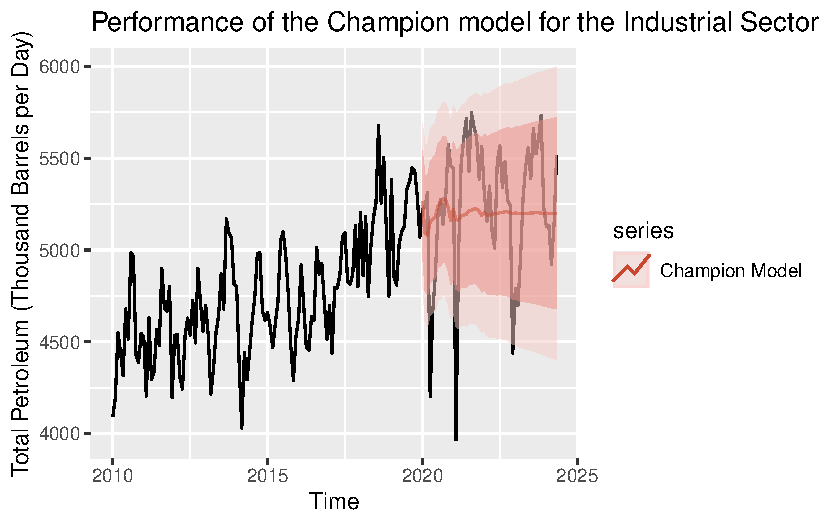
\includegraphics[keepaspectratio]{Report_files/figure-pdf/unnamed-chunk-32-1.pdf}}

From the above plot, it can be observed that the total petroleum
consumption in the industrial sector exceeded the 95\% prediction
interval significantly on three occasions. However, in all other months,
it remained within the 95\% interval. Additionally, since these three
fluctuations did not occur consecutively, it is difficult to
definitively attribute them to the impact of the COVID-19 pandemic in
the long-term.

\begin{verbatim}

Forecast method: ARIMA(1,1,1)(1,0,0)[12]

Model Information:
Series: Full_Dataset_industrial 
ARIMA(1,1,1)(1,0,0)[12] 

Coefficients:
         ar1      ma1    sar1
      0.4296  -0.9201  0.3121
s.e.  0.0967   0.0359  0.0951

sigma^2 = 47467:  log likelihood = -809.05
AIC=1626.09   AICc=1626.44   BIC=1637.21

Error measures:
                   ME     RMSE      MAE       MPE     MAPE      MASE
Training set 37.81642 214.2075 166.6114 0.6190439 3.494147 0.7251788
                    ACF1
Training set -0.06973329

Forecasts:
         Point Forecast    Lo 80    Hi 80    Lo 95    Hi 95
Jan 2020       5262.564 4983.353 5541.775 4835.547 5689.580
Feb 2020       5094.438 4781.069 5407.808 4615.181 5573.696
Mar 2020       5079.516 4755.228 5403.804 4583.561 5575.471
Apr 2020       5150.411 4820.950 5479.873 4646.543 5654.280
May 2020       5169.148 4836.308 5501.988 4660.113 5678.183
Jun 2020       5179.256 4843.696 5514.815 4666.062 5692.450
Jul 2020       5242.430 4904.419 5580.440 4725.488 5759.372
Aug 2020       5253.459 4913.117 5593.801 4732.951 5773.967
Sep 2020       5277.928 4935.314 5620.543 4753.945 5801.912
Oct 2020       5273.236 4928.382 5618.090 4745.827 5800.645
Nov 2020       5230.109 4883.037 5577.181 4699.308 5760.909
Dec 2020       5159.925 4810.653 5509.197 4625.760 5694.090
Jan 2021       5219.977 4848.581 5591.374 4651.975 5787.979
Feb 2021       5167.505 4786.831 5548.178 4585.315 5749.694
Mar 2021       5162.847 4776.637 5549.058 4572.190 5753.505
Apr 2021       5184.974 4794.540 5575.408 4587.857 5782.091
May 2021       5190.822 4796.687 5584.956 4588.045 5793.598
Jun 2021       5193.976 4796.371 5591.582 4585.891 5802.062
Jul 2021       5213.693 4812.727 5614.659 4600.469 5826.918
Aug 2021       5217.136 4812.872 5621.399 4598.867 5835.404
Sep 2021       5224.773 4817.252 5632.293 4601.524 5848.021
Oct 2021       5223.308 4812.563 5634.053 4595.128 5851.488
Nov 2021       5209.848 4795.906 5623.789 4576.779 5842.917
Dec 2021       5187.943 4770.831 5605.056 4550.024 5825.862
Jan 2022       5206.686 4782.245 5631.126 4557.560 5855.812
Feb 2022       5190.309 4760.891 5619.726 4533.571 5847.046
Mar 2022       5188.855 4755.341 5622.369 4525.853 5851.858
Apr 2022       5195.761 4758.516 5633.006 4527.053 5864.469
May 2022       5197.586 4756.778 5638.394 4523.428 5871.744
Jun 2022       5198.571 4754.285 5642.857 4519.094 5878.048
Jul 2022       5204.725 4757.012 5652.437 4520.007 5889.442
Aug 2022       5205.799 4754.696 5656.902 4515.896 5895.701
Sep 2022       5208.182 4753.719 5662.646 4513.140 5903.225
Oct 2022       5207.725 4749.927 5665.523 4507.584 5907.867
Nov 2022       5203.524 4742.417 5664.632 4498.322 5908.727
Dec 2022       5196.688 4732.295 5661.080 4486.461 5906.915
Jan 2023       5202.537 4733.806 5671.269 4485.675 5919.400
Feb 2023       5197.426 4724.938 5669.915 4474.818 5920.035
Mar 2023       5196.973 4720.977 5672.968 4469.000 5924.945
Apr 2023       5199.128 4719.742 5678.513 4465.971 5932.284
May 2023       5199.697 4716.985 5682.410 4461.452 5937.942
Jun 2023       5200.005 4714.004 5686.005 4456.731 5943.278
Jul 2023       5201.925 4712.666 5691.184 4453.668 5950.182
Aug 2023       5202.261 4709.767 5694.754 4449.057 5955.464
Sep 2023       5203.005 4707.300 5698.710 4444.889 5961.120
Oct 2023       5202.862 4703.966 5701.757 4439.867 5965.857
Nov 2023       5201.551 4699.485 5703.616 4433.708 5969.394
Dec 2023       5199.417 4694.201 5704.633 4426.756 5972.078
Jan 2024       5201.243 4692.596 5709.889 4423.335 5979.151
Feb 2024       5199.647 4687.741 5711.554 4416.754 5982.541
Mar 2024       5199.506 4684.422 5714.589 4411.754 5987.258
Apr 2024       5200.179 4681.964 5718.393 4407.638 5992.719
May 2024       5200.356 4679.041 5721.672 4403.073 5997.640
\end{verbatim}

\begin{verbatim}
# A tibble: 3 x 7
  Month      Value Point_Forecasts Lower_95_CI Upper_95_CI Difference Outlier
  <date>     <dbl>           <dbl>       <dbl>       <dbl>      <dbl> <chr>  
1 2020-04-01 4203.           5150.       4647.       5654.      -947. Lower  
2 2021-02-01 3966.           5168.       4585.       5750.     -1202. Lower  
3 2022-12-01 4439.           5197.       4486.       5907.      -758. Lower  
\end{verbatim}

The three significant drops in oil consumption in the U.S. industrial
sector observed in April 2020, February 2021, and December 2022 can be
attributed to several events. On March 15, 2020, the COVID-19 pandemic
led to widespread lockdowns, halting industrial activities causing a
sharp decline in oil demand and even temporarily pushing oil prices into
negative territory (David, 2023). In February 2021, a severe winter
storm in Texas disrupted oil production and refinery operations,
resulting in a reduction in consumption (Flores \& McBrien, 2023). While
the direct cause is uncertain, in December 2022, concerns over a global
economic downturn, inflation, and geopolitical risks stemming from
Russia's invasion of Ukraine led to reduced oil demand, further
contributing to the decline in consumption. These overlapping factors
likely caused significant drops in oil consumption during these periods.
Although there was a significant drop in oil consumption in April 2020,
it returned to within the 95\% prediction interval in the following
month. This suggests that the initial impact of the pandemic on oil
consumption in the industrial sector was short-term, and the sector
began to stabilize relatively quickly after the initial shock.
Therefore, we look at the duration from January 2020 to December 2020 in
the table below to see the effect by COVID-19 pandemic more directly.

\subsection{Conclusion}\label{conclusion}

This report focused on examining the impacts of COVID-19 on energy
consumption patterns in the industrial sector using ARIMA models for
forecasting.

For the industrial sector, an ARIMA(1,1,1)(1,0,0){[}12{]} model was
employed to assess petroleum consumption trends during the pandemic. The
model indicated that, while the sector experienced notable drops in oil
consumption in specific months---namely, April 2020, February 2021, and
December 2022---these fluctuations resulted from a combination of the
pandemic's effects, weather disruptions, and geopolitical risks. Despite
these disruptions, the model demonstrated a swift recovery, with
consumption quickly returning to the forecasted range after each shock.
The overall forecast error remained low at 1.550\%, suggesting that the
pandemic's impact on industrial energy consumption was brief and largely
resilient.

In summary, while the industrial sector faced temporary consumption
shocks during the pandemic, these were short-lived, and energy usage
stabilized relatively quickly. This resilience highlights the sector's
adaptability, with additional fluctuations driven by factors beyond the
pandemic itself.

\subsection{Reference}\label{reference}

Colander, D., Goldberg, M., Haas, A., Juselius, K., Kirman, A., Lux, T.,
\& Sloth, B. (2009). THE FINANCIAL CRISIS AND THE SYSTEMIC FAILURE OF
THE ECONOMICS PROFESSION. Critical Review, 21(2-3), 249--267.
https://doi.org/10.1080/08913810902934109

David, J. ((2023, March 15). CDC Museum COVID-19 timeline.
https://www.cdc.gov/museum/timeline/covid19.html\#:\textasciitilde:text=March\%2015\%2C\%202020,restaurants\%20and\%20bars\%20to\%20close.

Flores, N. M., \& McBrien, H. (2023). The 2021 Texas power crisis:
Distribution, duration, and disparities. Journal of Exposure Science \&
Environmental Epidemiology, 33(1), 21-31.
https://doi.org/10.1038/s41370-022-00462-5

Hyndman, R. J., \& Athanasopoulos, G. (2021). Forecasting: Principles
and practice (3rd ed.). OTexts. https://otexts.com/fpp3/




\end{document}
